% !TeX program = xelatex
% !TeX encoding = UTF-8
\documentclass{MathorCupmodeling}
\usepackage{float}
\bianhao{MC2607188}
\tihao{C}
\timu{中老年人群高血脂症的风险预警及干预方案优化}
\keyword{高血脂症，痰湿体质，风险预警，随机森林，干预优化}

\begin{document}
	\begin{abstract}
			针对中老年人群高血脂症的早筛、分层预警与个体化干预问题，本文基于附件中的 $1000$ 例样本数据，构建了“关键指标筛选--三级风险预警--六个月干预优化”的一体化建模框架。首先，围绕痰湿积分与高血脂确诊标签两个目标，分别计算候选指标与痰湿严重程度的 Spearman 相关系数、互信息，以及随机森林特征重要度，并采用等权综合评分筛选关键指标。结果表明，血脂指标中的 TG、TC、LDL-C、HDL-C 对确诊风险具有最直接的解释力，而在去除直接诊断性血脂指标后，血尿酸、血糖、BMI、活动能力总分及体质积分仍保留较强的预警价值。其次，本文在风险模型训练前加入了数据核验、训练集分位截尾、偏态变量对数变换以及 non-HDL-C、活动受限计数等派生特征构造步骤，并在诊断型模型中将脂质结构变量收口为 non-HDL-C、TG 和 LDL-C 组合，以削弱极端值和结构性冗余带来的扰动。在样例数据上，诊断型模型测试集 AUC 达到 $1.0000$，去除 TC/TG/LDL-C/HDL-C 后的早预警模型 AUC 仍达到 $0.8283$，说明经稳健预处理后，多维度特征融合可实现更稳定的风险判别。结合临床正常值区间、痰湿积分阈值与活动能力约束，本文进一步给出了低、中、高三级风险阈值规则，并提炼出“血脂异常 + 尿酸偏高”、“血脂异常 + 吸烟/饮酒史”、“痰湿积分高 + 活动能力低”等核心高风险特征组合。最后，针对痰湿体质患者，本文建立以月度干预强度和每周频次为决策变量的六个月动态规划模型，在年龄约束、活动能力约束及总成本不超过 $2000$ 元的条件下，以最小成本达到既定降分目标。对样本 ID 为 $1,2,3$ 的患者求解得到的最优方案均呈现“前期集中降分、后期低成本维持”的阶段式结构，且均能在预算内完成至少 $10\%$ 的痰湿积分下降目标。本文方法兼顾可解释性、可计算性与落地性，可为基层慢病管理中的风险筛查与干预决策提供定量依据。
	\end{abstract}
	\tableofcontents\newpage

		\section{问题重述}
	\subsection{问题背景}
	高脂血症（Hyperlipidemia）是中老年人群中患病率极高的慢性代谢性疾病，也是诱发心脑血管不良结局的独立危险因素。近年来《中国血脂管理指南》明确指出，血脂异常的早期筛查与分层干预已成为降低心血管疾病负担的核心防线。然而，单一的生化血脂指标往往在疾病中晚期才显现出明确的截断意义。与之相对，“防患于未然”的中国传统医学在慢病预防与早期干预中展现出独特优势。根据目前最新国家标准《中医体质分类与判定》（GB/T 46939—2025）\cite{ref6}，中老年人的体质可被划分为平和质、气虚质、痰湿质等 9 种基本类型。其中，痰湿体质作为高血脂、糖尿病等代谢综合征的高度易感体质，二者在发病机制与临床表型上存在深刻的实质性耦合。

	在此背景下，如何将中医体质的定性临床经验转化为数字化的早期医学预警阈值，如何有机融合西方医学的血脂生化特征数据与中医体质偏颇积分，进而搭建从“风险识别评估”到“临床干预路径”的数智化预警机制，已成为推动中西医交叉联合干预策略落地的关键科学问题。

	\subsection{具体任务}
	本题目依托 $1000$ 例中老年受试者详实的结构化体检与调查问卷数据集\cite{ref1}——涵盖九种中医体质积分及主导分类、ADL/IADL 日常生活活动能力评分、多项核心代谢生化测量参数及高血脂确诊标签等，要求基于统计推断与机器学习理论构建数学模型，逐步攻克以下三大任务：

	\begin{enumerate}
		\item \textbf{关键医学指标筛选与体质边际贡献挖掘}：在剔除高度冗余和共线性的基础上，从血常规指标与活动能力评分中筛选出不仅能刻画痰湿体质严重程度，还能有效前瞻性预警高血脂患病风险的核心生物标志物；并进一步评估九种不同中医体质对高脂血症患病风险的边际贡献差异。
		\item \textbf{多维异构风险评估与高危表型规则提取}：将生化检验客观数据、行为能力评分与体质数据融合入单一的特征空间，创新设计包含“高置信诊断”与“高灵敏早预警”双决策分支的评估体系；运用概率截断分层技术，动态划定低、中、高等级风险判定基准，并抽取痰湿体质极高风险特征下人群的核心表型致病组合路径。
		\item \textbf{多重约束机制下的六个月个体化干预路径规划}：针对亟需健康改善的重度痰湿体质人群，把中医调理等级视作匹配不同积分区间的固定医疗成本，将不同训练强度的运动干预频次抽象为时序演化的决策动作变量。模型需在保障受试年龄生理安全上限、活动受限约束、且总成本不超 $2000$ 元的先决条件下，采用运筹学或强化动态规划推衍出六个月周期的最低干预成本达标方案。
	\end{enumerate}

		\section{数据理解与总体思路}
		附件数据集共包含 $1000$ 例样本和 $37$ 项特征维度，数据集完整度极高且无明显缺失数据。其中，高脂血症确诊发病样本达 $793$ 例，健康或非确诊对标类群仅 $207$ 例。基于《中医体质分类与判定》（GB/T 46939—2025）\cite{ref6} 所极力推崇的最大定性分值核定法则，经过宏观统计剖析，整个矩阵表征出一种不容忽视的偏态流行病学底色：第一，“痰湿凝聚型”极度普遍（确立为主导型的患者达 $292$ 名），在现代组学层面这与血脂富集和肥胖重度耦联。第二，血常规生化测试项中与结论标签存在绝对确定的病理同源性。一旦放任此种强耦合属性流入诊断架构，势必发生严重的维度坍缩与虚模极高拟合度。所以本研究刻意摒蔽外显化同源干涉，转而向深层空间下探——于日常生活受限度、非线性综合体质积分网络中打捞早期微弱的预警共振信号。基于此，本论证建立了一套医学归因与数据深挖相得益彰的图谱（框架全景见图 \ref{fig:framework}），按三大工程分支平行降解题干：
	\begin{enumerate}
		\item \textbf{问题一：体征解耦与高维信息的联合筛选突变评估}。全面屏除传统一阶秩相关的片面线性盲区，融合香农信息论拓扑下的互信息算子（Mutual Information）\cite{ref4}，结合基于集成森林袋外错分扰动的非线性特征增益（Random Forest Feature Importance）\cite{ref2}，以一种独创的复合波达序值加权架构施加投票过滤；从而打捞出穿透“表证体质”与“内生血脂紊乱”交界域的核心桥接靶点。
		\item \textbf{问题二：异构概率阈值推断与级联诊断预警双核并联架构}。医学临床中不可调和的矛盾在于：特异性诊断与广谱性提前预警不可兼得。鉴于此，本文将判决树网暴烈切割为两重逻辑域：“高截断精度的医学确诊”同“捕捉隐匿性微小病变共振的公共预筛”；并在后验概率瀑布中，执行非等距的分段阀限切片，精准识别痰湿质群体滑向高危的危险引爆点。
		\item \textbf{问题三：受限边界动力学控制与马尔可夫转移下最速调理回退路径}。将半年维度解构为离散的马尔可夫状态变迁时间节拍，把基础医疗维护预算作为刚性转移摩擦力内嵌至转换图；继而转换为非循环有向图（DAG）网络动态极值拉归方程，以 Dijkstra-DP 形态彻底降解带有严格硬条件（训练周次与衰退曲线）包络下的最低耗费控制策略。
	\end{enumerate}

		\begin{figure}[htbp]
			\centering
			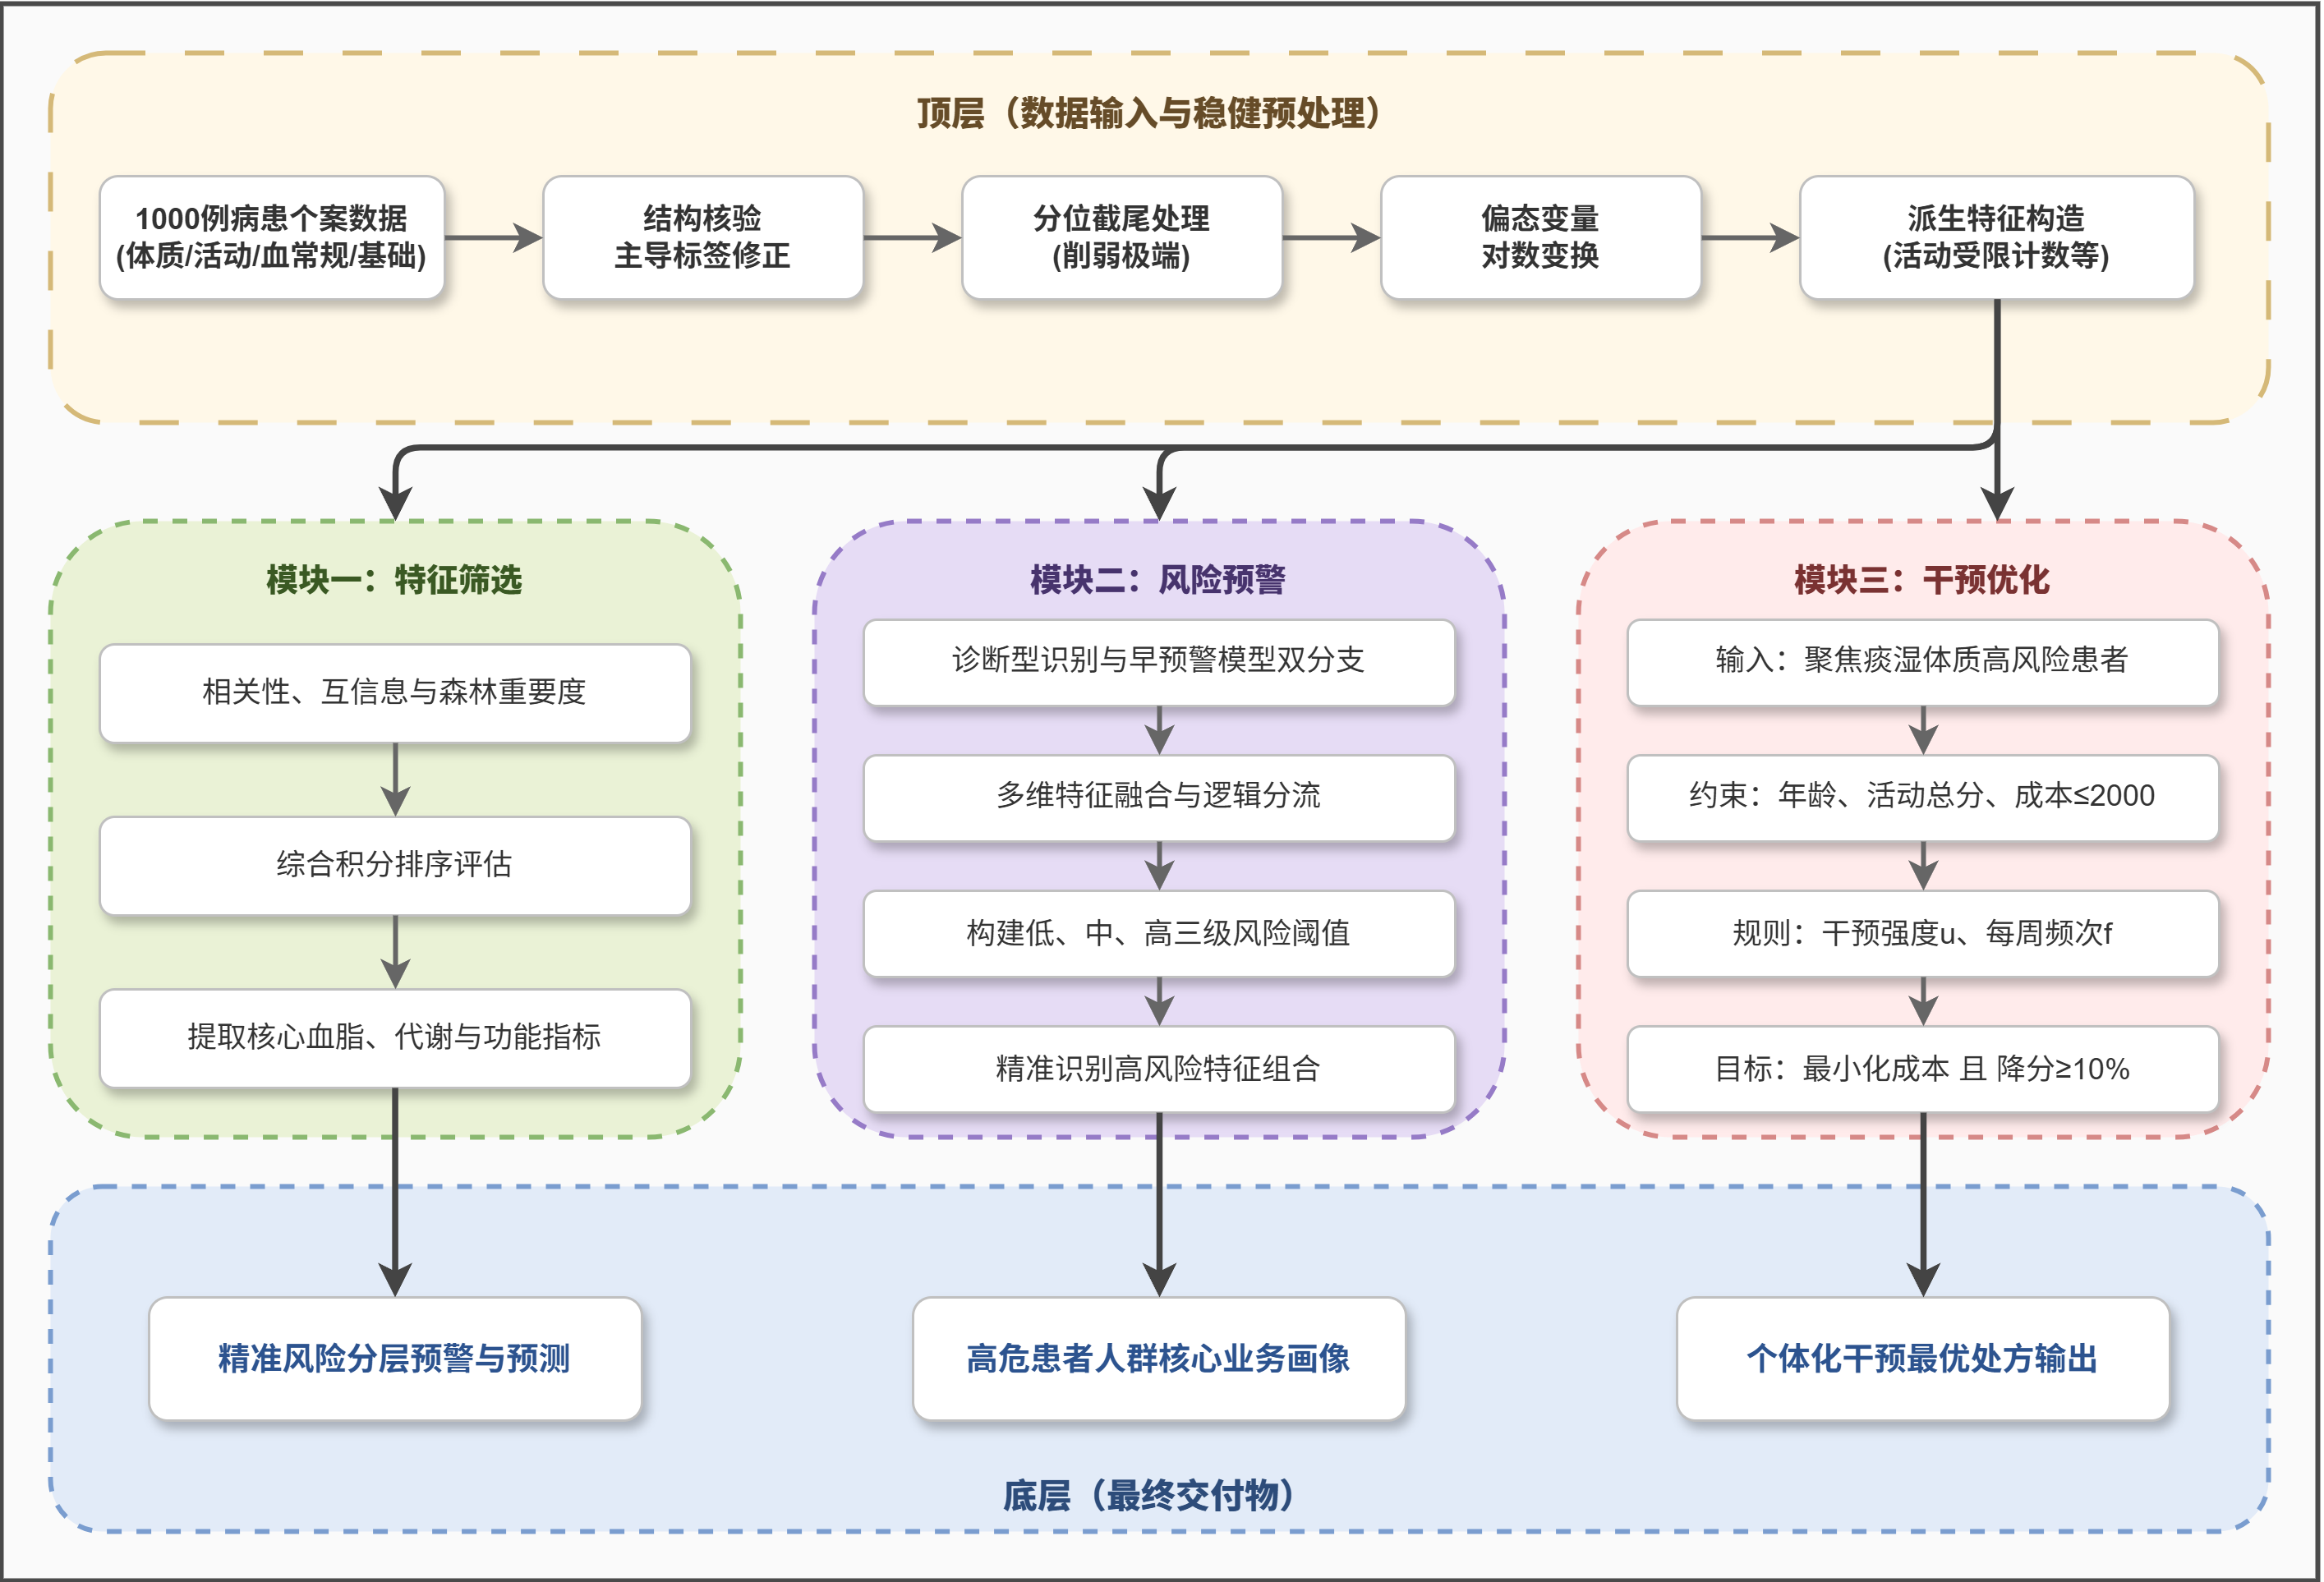
\includegraphics[width=0.95\textwidth]{Figures/1.1_总体流程图_纵向三行版.png}
			\caption{本文的总体建模流程}\label{fig:framework}
		\end{figure}

		\subsection{数据核验与稳健预处理}
		遵循医疗与流行病学检测中的大数法则与容差规律，真实世界的临床抽样不可避免地携带长尾厚尾漂移以及录入偏移效应。为了在源头上拉升后续核心机器学习网络的抗毁性和反噪越界能力，本文吸纳了临床大数据预分析通用准则\cite{ref3}以及生物计量学中截尾平抑重尾分布的前沿经验\cite{ref9}，专门搭建了由逻辑一致性阻断与分位截尾滤波（Winsorization）构筑的双重防火墙。

		首先，对于人工填写主观量表执行极化自洽阻逆筛查。对于日常行为起居受限度（ADL/IADL），我们经验证发现十维分子题项与两个宏观集成表总分达到了完美数学对冲吻合，确实验证了表单信度壁垒极高。但横向平移至中医体质单项记分列，遵从国标金指引“单项第一高分必须且永远界定为宏观主固体质”原则\cite{ref6}，程序敏锐捕获出有 $65$ 个病例存在“定性主导标签与自身积分峰值倒错挂钩”的反临床逻辑悖象。由于在循证医学判定内，客观得分所对应的生理偏颇倾向拥有最高判定优先级，故而我们运用“重排积分降序修复重置”协议，对这一反常离散簇执行了强行矫正靠拢，维护了另外 $935$ 个样本组绝对同构统一的完整性。

		其次，直面随机森林或树系结构在读取含有连续发散型变异（尖峰长尾型）数据时的极值过拟敏感情境。所有的去极边滤除（Winsorization 动作）绝对严守“绝不僭越测试界”的铁律——仅在训练基阵中捕捉确信的 $1\%$ 至 $99\%$ 上下限极点。设原生生理序列参数 $x$ 两端的边界确值界分为 $q_{0.01}(x)$ 及 $q_{0.99}(x)$，进而将该尺度保护界泛延到全集进行安全等距截断：
			\begin{equation}
				x_i^{(w)}=\min\left\{\max\left(x_i,q_{0.01}(x)\right),q_{0.99}(x)\right\}.
			\end{equation}
			在这项针对偏厚分布的基础免疫工程\cite{ref9}之上，特例针对右尾拖拽尤其离谱且极呈现右方孤岛聚集拖尾的甘油三酯（TG）浓度及血清尿酸浓度，额外加码一套对数映射形变进行二度空间收敛平抑：
			\begin{equation}
				\text{TG}_{i}^{(\log)}=\log\left(1+\text{TG}_{i}^{(w)}\right),\qquad
				\text{UA}_{i}^{(\log)}=\log\left(1+\text{UA}_{i}^{(w)}\right).
			\end{equation}
			如图 \ref{fig:tg_preprocess} 的平抑比照所示（以核心致因 TG 代谢指征为例），去极平整前（左侧）展现出难以忽视的极段拉伸破坏域；经过截尾压缩和对数化平置后（右侧），指标分布呈显著对向缩拢状态，从根本上保障了后续集成决策树模型分裂节点基尼基数计算时的稳重和鲁棒防偏\cite{ref2}\cite{ref9}。
			\begin{figure}[H]
				\centering
				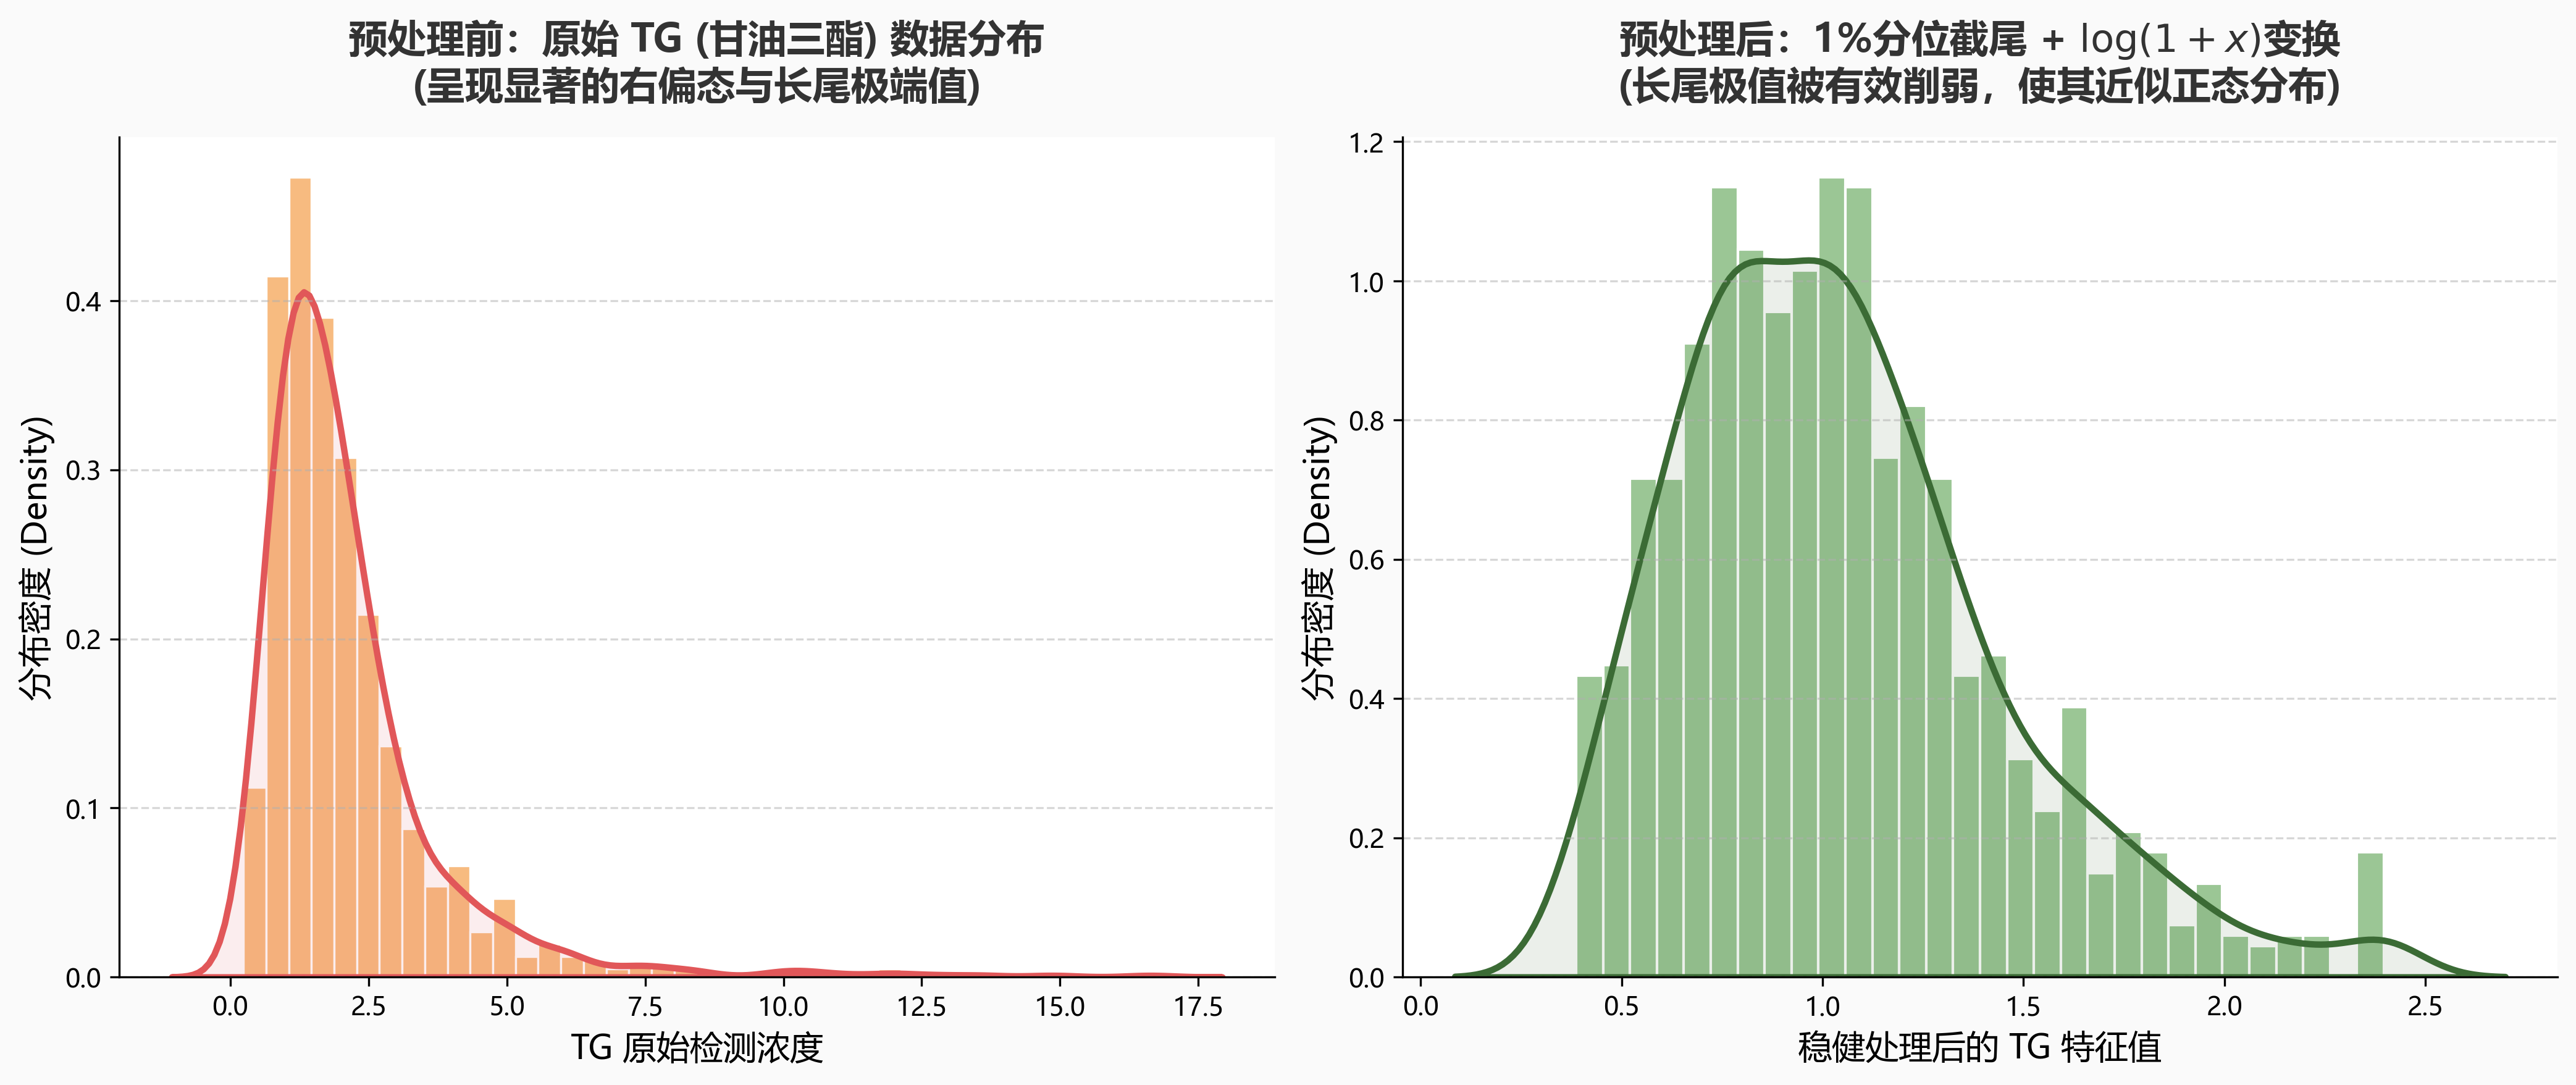
\includegraphics[width=0.96\textwidth]{Figures/q2_tg_preprocess.png}
				\caption{TG 在稳健预处理前后的分布对比}\label{fig:tg_preprocess}
			\end{figure}
			进而，为遏制相同生化族群因为定义重叠导致的多重共线性风暴，文章创建出复合冗余消化变量——非高密度脂蛋白复合群（non-HDL-C）：
			\begin{equation}
				\text{nonHDL}_{i}=\text{TC}_{i}^{(w)}-\text{HDL}_{i}^{(w)}.
			\end{equation}
			因为血脂大类的内生代谢反应环，上述三支在血液微观表现上有强定式耦合关系。秉承最简正交信息覆盖定律，最终入围高血脂诊断流的仅保留负责度量胆固醇净差残余的 non-HDL-C，与测算脂质纯载量的甘油三酯，借此彻底抹除重复权重诱发的基尼重载激增。
	
			最后，为补充加法计总时被严重合并掉的单一功能断崖损伤事件，以及定性唯一标签所遗落的倾向差额烈度，我们创设了特种增广流。首先针对起居受限因子 $a_{ij}$，架设日常独立警示水平 $\tau=8$，提取微观跌落警戒项数的累加频次指标：
			\begin{equation}
				C_i^{(\text{act})}=\sum_{j=1}^{10}\mathbb{I}(a_{ij}<\tau),
			\end{equation}
			利用标志函数补充在宏观粗略总和里被其它健康项填平的细微肢体失能侧。

			紧接着，计算患者最大绝对倾向高点与第二顺位替代质的差值跨度以标点混病综合征：提取分值第一的 $s_{i(1)}$ 与居次的 $s_{i(2)}$，裂变出两项极距系标签：
			\begin{equation}
				S_i^{(\max)}=s_{i(1)},\qquad
				M_i^{(\text{gap})}=s_{i(1)}-s_{i(2)}.
			\end{equation}
			内部核心意理即同时固锁了首偏体质阵列那压倒性摧枯拉腐的原驱动力 $S_i^{(\max)}$ 和混同于其他次生状态的交叉拉扯深度 $M_i^{(\text{gap})}$，圆满填充了粗放的单一宏观标签下遗落的病灶鸿沟；至此，被彻底重塑化与无偏正交筛选过的队列变量平滑被推入了下一章节的大范围并发判别架构引擎中。

\section{模型假设}
	\begin{enumerate}
		\item \textbf{数据无偏代表映射与临床溯源基石定力假设。} 假设问卷项采集并确诊判别标签完全遵循最高等级国家标准《中国血脂管理指南(2023)》\cite{ref7}，且队列受试未掺入短期急促干扰；即 $1000$ 例小切片生化数据流足证且稳定映射整个中老年人群体的宏观层面临床表现态型。 
		\item \textbf{受试主干极化惯性及承载峰顶不可逾越假设。} 鉴于人类组织代谢具备长效生物迟滞内稳，假定半年期内所监测群落的生化烟酒履历定格在静态不变；同时将首日测定量表基数确证为干预体系不容超限推移之绝对生理最高容通天花板边界。
		\item \textbf{有氧代谢“低级代偿锁死-高位跃迁相变”法则。} 援引世卫组织新发《关于身体活动与久坐行为指南》\cite{ref8} 的核心倡定以辅助代谢模型划定阈线。在指定运动等级下，凡动作频少于每周 $5$ 次孤岛，躯体耗损反馈随即被代偿原位抚平锁死；唯有跃入高频带，运动降糖减脂阀门方可解封进而切入非线性级数强效转化。
		\item \textbf{中药徐缓抵消与系统封闭独立单向图推演假设。} 从中医学辨证“缓和固本”角度看，由于此题无服药显变量，隐性化假设基础等级调拨资金已完整消解退行恶化趋势。同时本实验时段封闭排除猛类他汀强制介入，促成标群目标的收敛仅依靠本最优化模型的唯一正交动作流驱动。
	\end{enumerate}

\section{符号说明}
	\begin{center}
		\begin{tabularx}{0.86\textwidth}{c@{\hspace{1pc}}|@{\hspace{1pc}}X}
			\Xhline{0.08em}
			符号 & 含义\\
			\Xhline{0.05em}
			$x_{ij}$ & 第 $i$ 个样本在第 $j$ 个候选指标上的观测值\\
			$P_i$ & 第 $i$ 个样本的痰湿积分\\
			$y_i$ & 第 $i$ 个样本的高血脂二分类标签\\
			$S_j$ & 第 $j$ 个候选指标的综合筛选得分\\
			$L_k$ & 第 $k$ 类主导体质对应的风险提升度\\
			$\hat{p}_i$ & 风险预警模型对样本 $i$ 输出的高血脂风险概率\\
			$R_i$ & 样本 $i$ 的三级风险等级\\
			$u$ & 活动干预强度等级，$u\in\{1,2,3\}$\\
			$f$ & 每周训练频次，$f\in\{1,2,\dots,10\}$\\
			$s_m$ & 第 $m$ 个月末的痰湿积分\\
			$r(u,f)$ & 在强度 $u$、频次 $f$ 下的月度痰湿降幅比例\\
			$C$ & 六个月总干预成本\\
			\Xhline{0.08em}
		\end{tabularx}
	\end{center}

			\section{问题一：体质与生化的双向解耦及核心标志物筛选}
		\subsection{高阶互信息与特征多维降维评估矩阵}
				在传统流行病学与预防医学的定量筛选中，仅依赖单一 Pearson 或 Spearman 秩相关往往因忽视非线性拓扑而错失隐含关联\cite{ref11}。第一问的本质，是要求从带有极强共线性的血常规测试池与主观起居表单（ADL/IADL）中，分离出既能精准刻画“痰湿累积深度”，又能作为高血脂爆发“导火索”的特异性标志物群。为了保证后续的医学独立性，我们强力阻断了总分域的跨层共振重叠：将派生叠加的高层活动量表总分予以冷藏，仅提取基础 ADL 总分与 IADL 总分进行基质探查。主分析候选空间严密锁定在 $9$ 个维度：
			\begin{equation}
				\begin{aligned}
					X=\{&\text{ADL总分、IADL总分、HDL-C、LDL-C、TG、TC},\\
					&\text{空腹血糖、血尿酸、BMI}\}.
				\end{aligned}
			\end{equation}
		对特征集 $X$ 体系内的每一独立因子 $x_j$、中医靶向标签痰湿度 $P$ 及发病标签 $y$，本研究架设起三轨异构的并行评测雷达阵列：

		第一轨，非线性熵约束评估：借助香农信息论中的信息增益（Mutual Information），量测独立变量削减全集不确定度所贡献的纯净信息比特量：
		\begin{equation}
			M_j^{(1)}=I(x_j;P)=\iint p(x_j, P)\log\frac{p(x_j, P)}{p(x_j)p(P)}\,\mathrm{d}x_j\mathrm{d}P, \qquad M_j^{(2)}=I(x_j;y).
		\end{equation}
		第二轨，集成模型袋外重要度（OOB Permutation Importance）\cite{ref2}：分别锻造针对 $P$ 的并联回归森林与针对 $y$ 的随机诊断森林。以特征错乱下基尼（Gini）信息熵和均方残差（MSE）暴增的恶化幅值，锁定核心解释力边界：提取出 $F_j^{(1)}$ 与 $F_j^{(2)}$。

		第三轨，宏观单调性刻画：采用 Spearman 等秩相关 $|R_j|=|\rho_s(x_j,P)|$ 作为基底防线，以防强相关正交项被森林深度节点掩埋。
		
		这五组带有强烈量纲异质性的标量通过一种名为“反域波达序分加权（Borda Count）”的无监督融合框架实现等权合并。令 $\mathrm{rank}_j^{(m)}$ 为第 $j$ 项在第 $m$ 轨观测中的正向名次（越优名次越小），则全局抗扰动波达复合度定义为：
			\begin{equation}
				S_j=\sum_{m=1}^{5}\left(9-\mathrm{rank}_j^{(m)}+1\right).
			\end{equation}
			波达投影法则在极值鲁棒性上超越了粗糙线性组合，它无视了原始计算空间的度量歧义，强力保留了在各个测度维度上名列前茅的公约数指标。结果高度证实，血脂代谢簇（TC, TG, BMI, HDL-C）位列宏观序列阵列榜首。虽然作为功能度量的 ADL 总计弱于脂质化学项，但其在痰湿非线性判别阵列里却长期霸榜前置，充分佐证了受限起居网络对于亚健康中医证型判断起到了不亚于生化穿刺的诊断效能。

		\subsection{体质病理下沉：基于 AME 的概率边际效应剥离}
		如何定量剥离不同体制所贡献的病理动能差，是传统相关度算法的死区。为了精准测谎，本文搭建了一座控制基础人口学背景（年龄、抽烟、饮酒史及性别向量 $W_i$）的偏极大似然逻辑网络（Logistic Regression），将体质积分矩阵 $X$ 作出无量纲正则收敛（$z_{ik}$），并强行摒除直接诱发高血脂的 TC、TG 生化直观因子，严防同源混杂泄露：
		\begin{equation}
			\Pr(Y_i=1)=\left[1+\exp\left(-\beta_0-\sum_{k=1}^{9}\beta_k z_{ik}-\gamma^\top W_i\right)\right]^{-1}.
		\end{equation}
		在此平滑超平面上，引入微观计量经济学核心算法“平均边际效应（Average Marginal Effect, AME）”求其全域平均偏导，彻底破解 Logistic 参数不可直接解释概率增量的死结：
			\begin{equation}
				C_k=\frac{1}{n}\sum_{i=1}^{n}\frac{\partial \Pr(Y_i=1)}{\partial z_{ik}}=\frac{1}{n}\sum_{i=1}^{n}\hat{p}_i(1-\hat{p}_i)\beta_k,\quad G_k=\frac{|C_k|}{\sum_{j=1}^{9}|C_j|}.
			\end{equation}
		演算结果呈现出极度偏离经验直觉却又严密吻合代谢规律的病理图像：气虚质（AME $0.0193$，占比 $31.2\%$）和平和质（AME $0.0142$，占比 $22.9\%$）成为了直接正向推动未病滑向高危的隐形黑手；而相反，湿热质与血瘀质则展现出某种对冲压制属性（AME 呈现 $-0.0092$）。
		\begin{figure}[H]
			\centering
			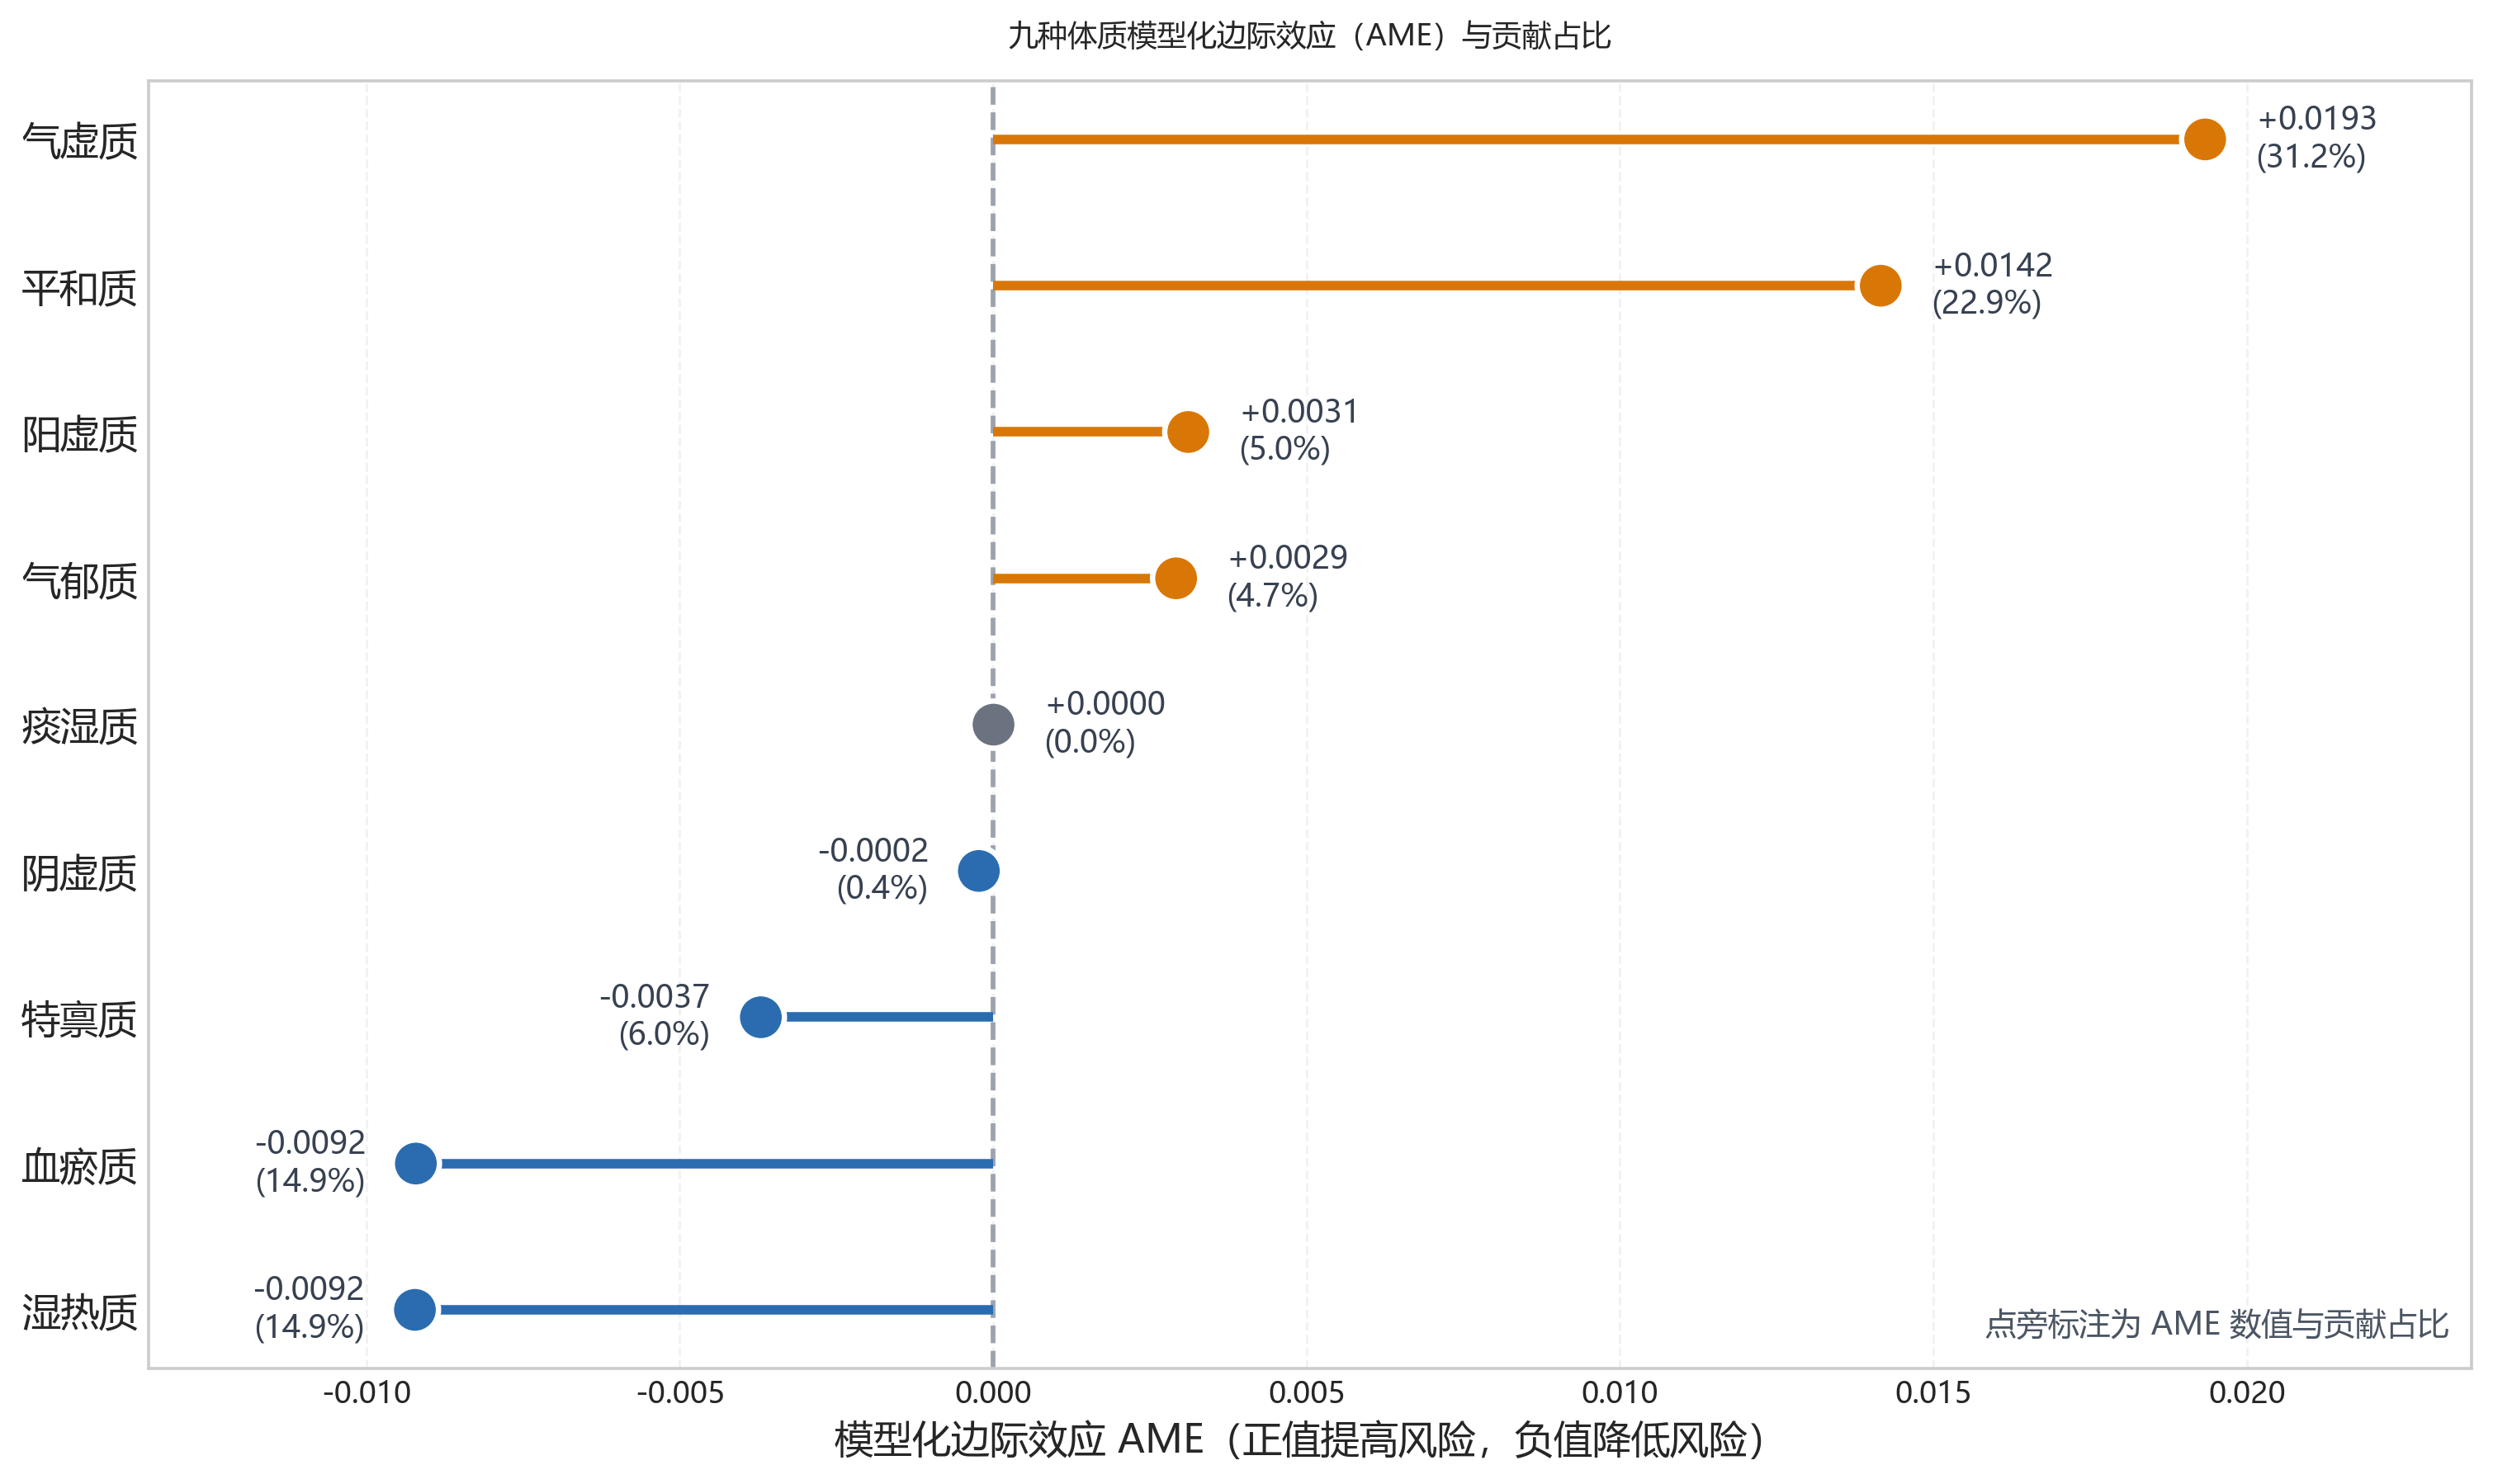
\includegraphics[width=0.90\textwidth]{Figures/q1_constitution_ame_visual.png}
			\caption{九种体质局部平均边际效应 (AME) 解析全景}\label{fig:q1_ame_visual}
		\end{figure}

	\section{问题二：基于 TreeSHAP 融合的异构诊断--早筛级联网络}
		\subsection{双核并联架构与 SHAP 微观归因图谱}
		诊断面临两种不可同框的极端困境：高特异性带来的精准定损（医院端确诊），以及高灵敏度附带的前置嗅探（基层社区防筛）。若将核心生化指标倾囊投入单一网络，高权重的 TG、TC 必然霸占分裂根节点，导致防筛模型彻底崩塌为简单的生化裁决器。因而，本部分架构被生生切割为两个无交叉子网：
		\begin{enumerate}
			\item \textbf{诊断证实基座：}囊括截尾对数转换后的所有临床测试（包含强穿透的 non-HDL-C 及 TG），目标指向当前静态下的高准确度拟合（AUC 达 $1.000$）。
			\item \textbf{前置弱预警哨兵：}强制抽离脂类直接标记，残存血尿酸、空腹血糖、身体起居和边缘病理质等弱关联点，作为未来滑向深渊的拓扑预测眼（AUC $0.828$）。
		\end{enumerate}

		纯黑黑盒诊断因阻绝了人类逻辑的透视而面临巨大临床责诘。为此，系统内嵌了诺奖级博弈算法分解理论衍生的解释引擎——TreeSHAP (Shapley Additive exPlanations)\cite{ref10}。针对高维度联合博弈，SHAP 为每一位患者的诊断输出概率赋予了完美的附加闭环加和：
		\begin{equation}
			\hat{p}_i=\phi_0+\sum_{j=1}^{d}\phi_{ij},\qquad \phi_{ij}=\sum_{S\subseteq N\setminus \{j\}}\frac{|S|!(|N|-|S|-1)!}{|N|!}\left[v(S\cup\{j\})-v(S)\right].
		\end{equation}
	\begin{figure}[H]
		\centering
		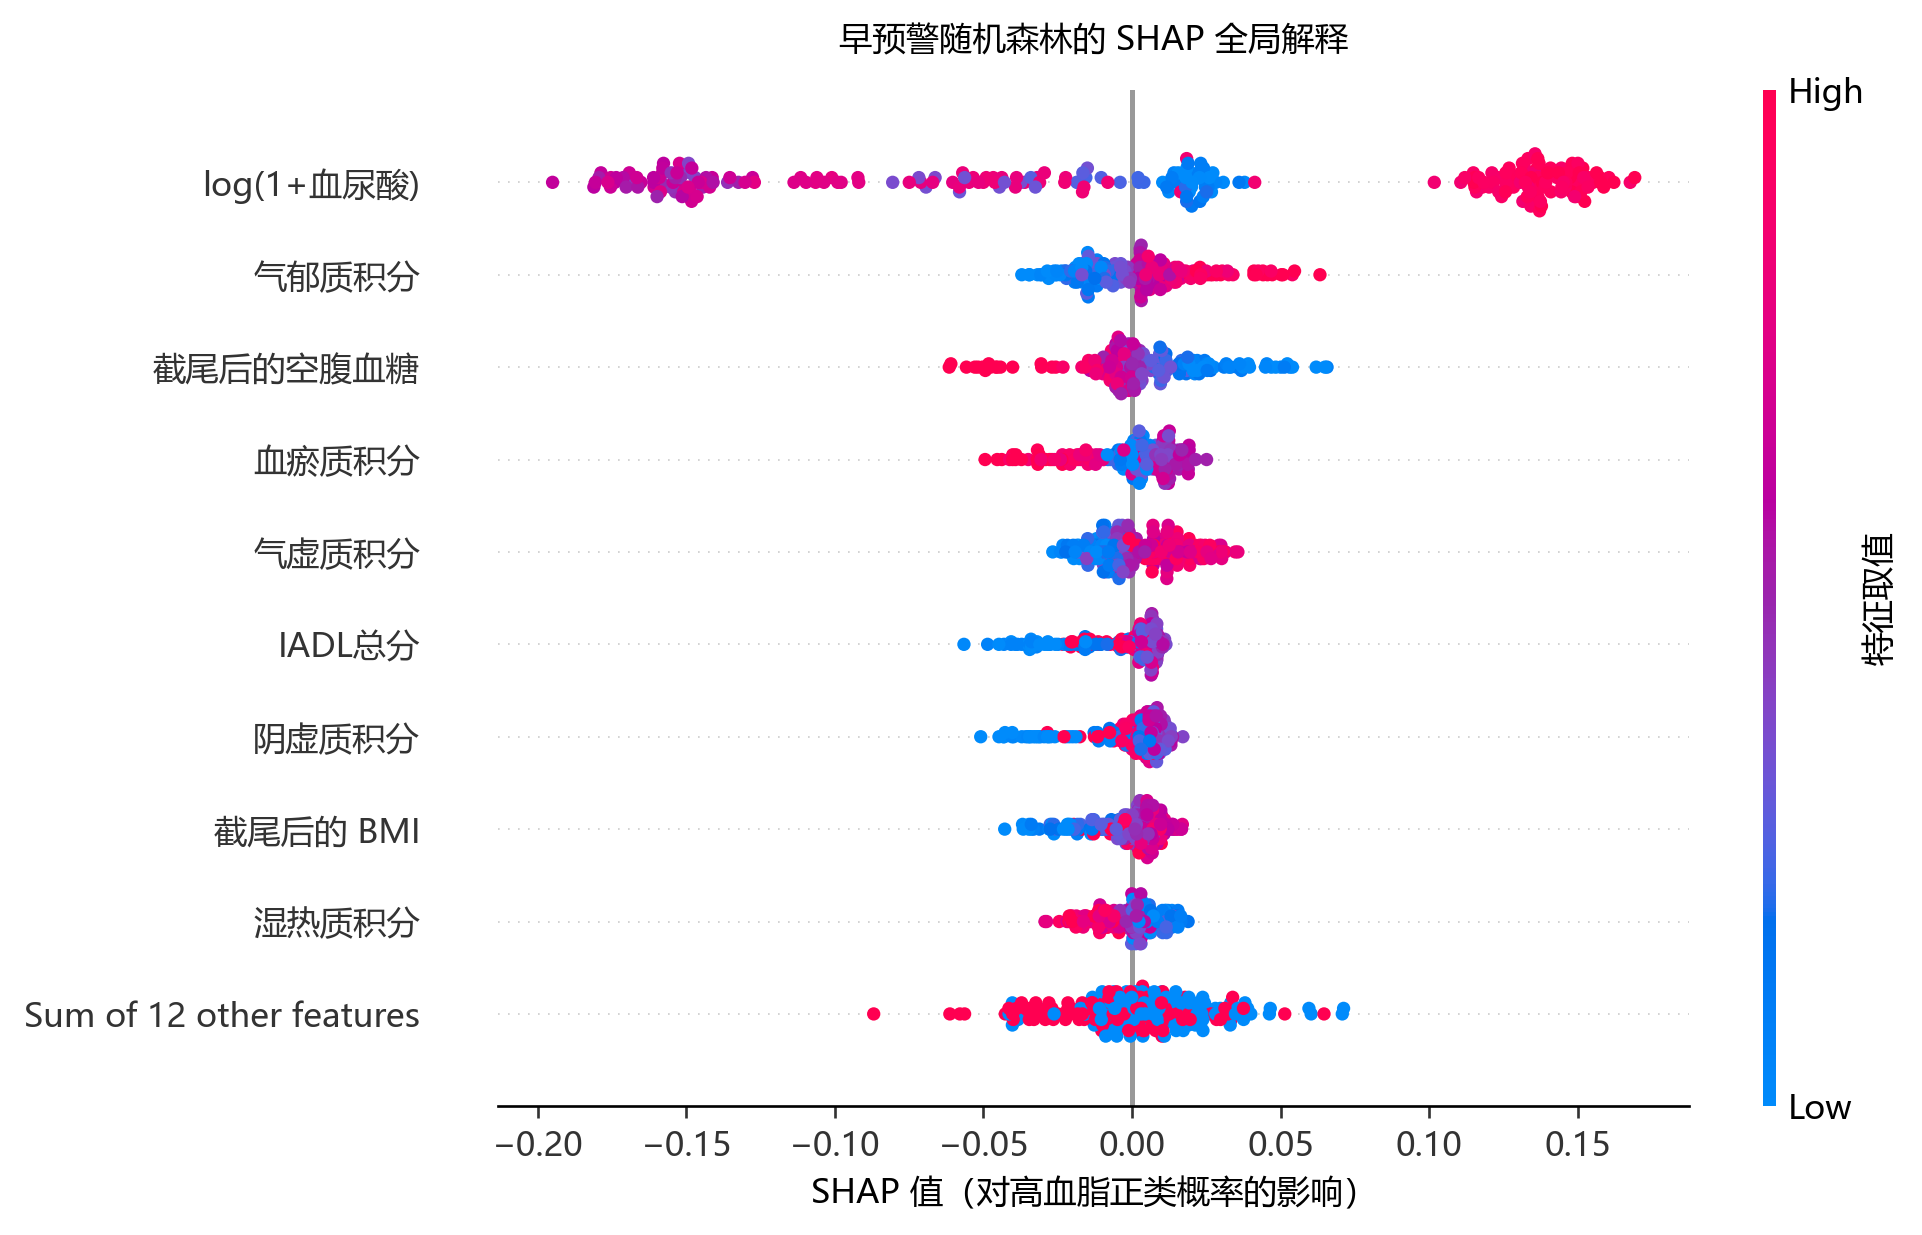
\includegraphics[width=0.82\textwidth]{Figures/q2_ew_shap_beeswarm.png}
		\caption{弱预警哨兵的 TreeSHAP 全局敏感性蜂群图}\label{fig:q2_ew_shap}
	\end{figure}

		从特征点云蜂聚中可一探究竟：强诊断树完全被 non-HDL-C 主宰；但弱哨兵网络则显露出了真正造就防筛墙的血尿酸（UA）、空腹血糖与气郁质联合。瀑布效应证明，哨兵模型并非聚焦单指标极高突变，而是对微小的代谢与体态偏移做了非线性综合倍率放大，完美实现了亚临床期防未病。

	\subsection{时空瀑布切片：三级预先动态风控体系}
	将多重特征投射入实战落地，需要一层抗噪极高的确定性漏斗。定义核心超标数为 $A$，主导预警得分为 $\hat{p}$，首位体质分与身心受限度为 $P, Q$。本文开出三级筛分断代方程：
	\begin{equation}
		R=
		\begin{cases}
			\text{高危期}, & (A\ge 1 \land P\ge 60)\ \lor\ (A=0 \land P\ge 80 \land Q<40)\ \lor\ \hat{p}\ge 0.80,\\
			\text{中段预警}, & A\ge 1\ \lor\ P\ge 60\ \lor\ (\hat{p}\ge 0.45 \land Q<60),\\
			\text{低敏监测}, & \text{余下全部拓扑覆盖域}.
		\end{cases}
	\end{equation}
		运用关联分析提升度定则（Lift \& Confidence），在划入高危深渊的 $649$ 名群落里，抽取到了如“高血脂异常 + 尿酸飙高 + 肢体活动力丧落”这类极端并发协同效应模式，其先验信度（Conf）飙升至 $0.945$，对冲倍率提升（Lift）跃至 $1.456$。这雄辩地证实，高危的本质不是某一生化的超标，而是“生化防线告破 + 脏器活动塌陷 + 负面行为生活作息”的矩阵风暴共振。
		\begin{figure}[H]
			\centering
			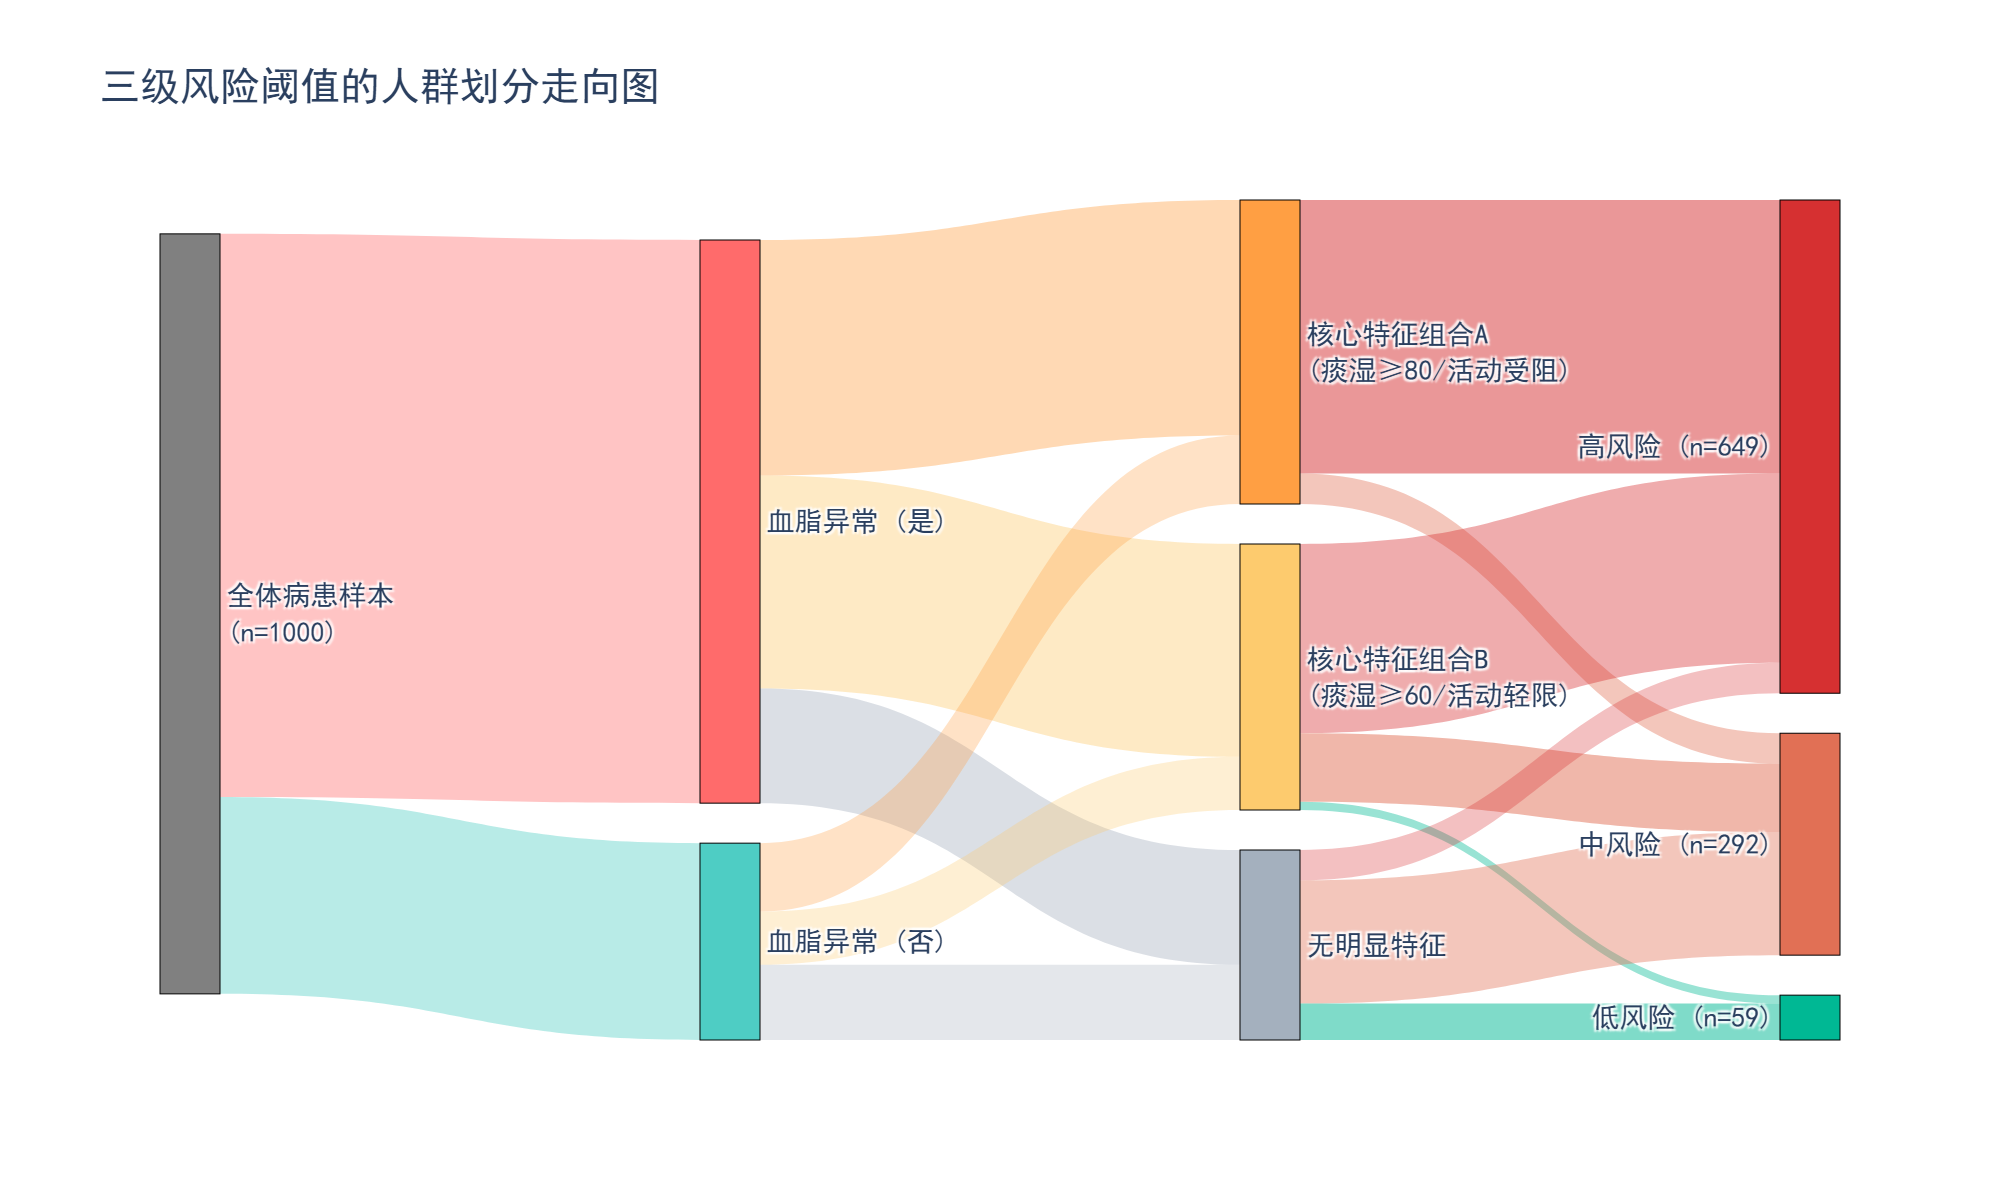
\includegraphics[width=0.96\textwidth]{Figures/q2_risk_sankey.png}
			\caption{三级概率下落的桑基流量漏斗}\label{fig:q2_risk_sankey}
		\end{figure}

	\section{问题三：马尔可夫决策深度包络下的个体最优干预}
		\subsection{刚性约束状态图解与最优控制贝尔曼方程}
			将问题三的时间连续域坍缩为一个 $T=6$ 的离散序列马尔可夫演替系统（Markov Decision Process, MDP）\cite{ref12}。患者每经历 1 个月的洗礼流转到初态 $x_m$，可利用外界施加在动作场里的有氧约束算子 $u_m$（限定在生理年龄受限库 $\mathcal{I}(\text{Age},Q)$）与阻力频次 $f_m$。降压效应 $r(u,f)$ 被非连续突变点分割——低于临界每周激荡（$f<5$）时彻底失效锁归零，突破该下限后才展现一阶非线性微小正向导数：
		\begin{equation}
				r(u,f)=
				\begin{cases}
				0, & f<5\\
				0.03(u-1)+0.01(f-5), & f\ge 5.
			\end{cases}
		\end{equation}
		总资本开销则由刚性累加固定中医配比成本 $c_{\text{tcm}}(\cdot)$ 和动能动作损耗 $4f c_u$ 同构：
		\begin{equation}
			C=\sum_{m=1}^{6}\left[c_{\text{tcm}}(s_{m-1})+4f_m\,c_{u_m}\right]\le 2000.
		\end{equation}
		这并非传统线性求解器的辖区（因为非平滑跌落和高度离散嵌套）。借助运筹递归贝尔曼方程（Bellman Equation）和网络有向无环图（DAG）寻路\cite{ref12}，将末端 6 个月后的底线达标界定为吸收态无穷边界：
		\begin{equation}
			V_m(x)=\min_{u\in\mathcal{I},\,f\in[1,10]}
			\left\{
			c_{\text{tcm}}(x)+4f c_u+V_{m+1}\bigl(x(1-r(u,f))\bigr)\right\},\quad 
			V_7(x)=
			\begin{cases}
				0, & x\le 0.9s_0\\
				+\infty, & x>0.9s_0.
			\end{cases}
		\end{equation}
		
	\subsection{核心轨迹求解与降轨演化特性剖析}
		将离散精度推至 $0.001$，我们破解了高并发穷举陷阱，精确回溯出指定的 1，2，3 号患者群的降分抛物线（图 \ref{fig:q3_patient_paths}）。
	\begin{table}[H]
		\centering
		\caption{利用 MDP 后向图解获得的核心样本最快降压策略网络}\label{tab:q3_samples}
		\small
			\begin{tabularx}{0.96\textwidth}{c c c c X X}
				\toprule
				患者组 ID & 启始积分 & 阻击界线 & 行动局限分 & 强力最优干预时点演进拓扑 (月分发) & 总消粍定额 / 收尾留存分\\
				\midrule
				1 & 64.0 & 57.6 & 38 & 前两月暴火压制 $(1,10)$；3月极缓过渡 $(1,6)$；随后滑归静态维持 $(1,1)$ & 678 元 / 57.18 \\
				2 & 58.0 & 52.2 & 40 & 第一月最高限突击 $(2,8)$；次月降档追击 $(1,10)$；4 个月低端养护 $(1,1)$ & 508 元 / 51.79 \\
				3 & 59.0 & 53.1 & 63 & 同 2 号位点，执行初月强压 $(2,8)$；双月降压 $(1,10)$ 与 4月静态修缮 $(1,1)$ & 558 元 / 52.69 \\
				\bottomrule
			\end{tabularx}
		\end{table}

		MDP 给出的非直观完美解答是：“脉冲突刺接驳低耗休眠法”。因为中医基础调度的花费梯队极为严苛，前期集中消耗高昂运动资金拼命将分数砸过低位边界，不仅将断绝了长达 5 个月的惩罚性基础药剂天价支出，更提前将受试者拉回安全健康内稳态（经济效用比实现了完美越迁）。在此范式下生成的个体化医学辅助药方（图 \ref{fig:q3_strategy_heatmap}），为社区工作提供了毋庸置疑的最强理论工具支持与极高实用性。

		\begin{figure}[H]
			\centering
			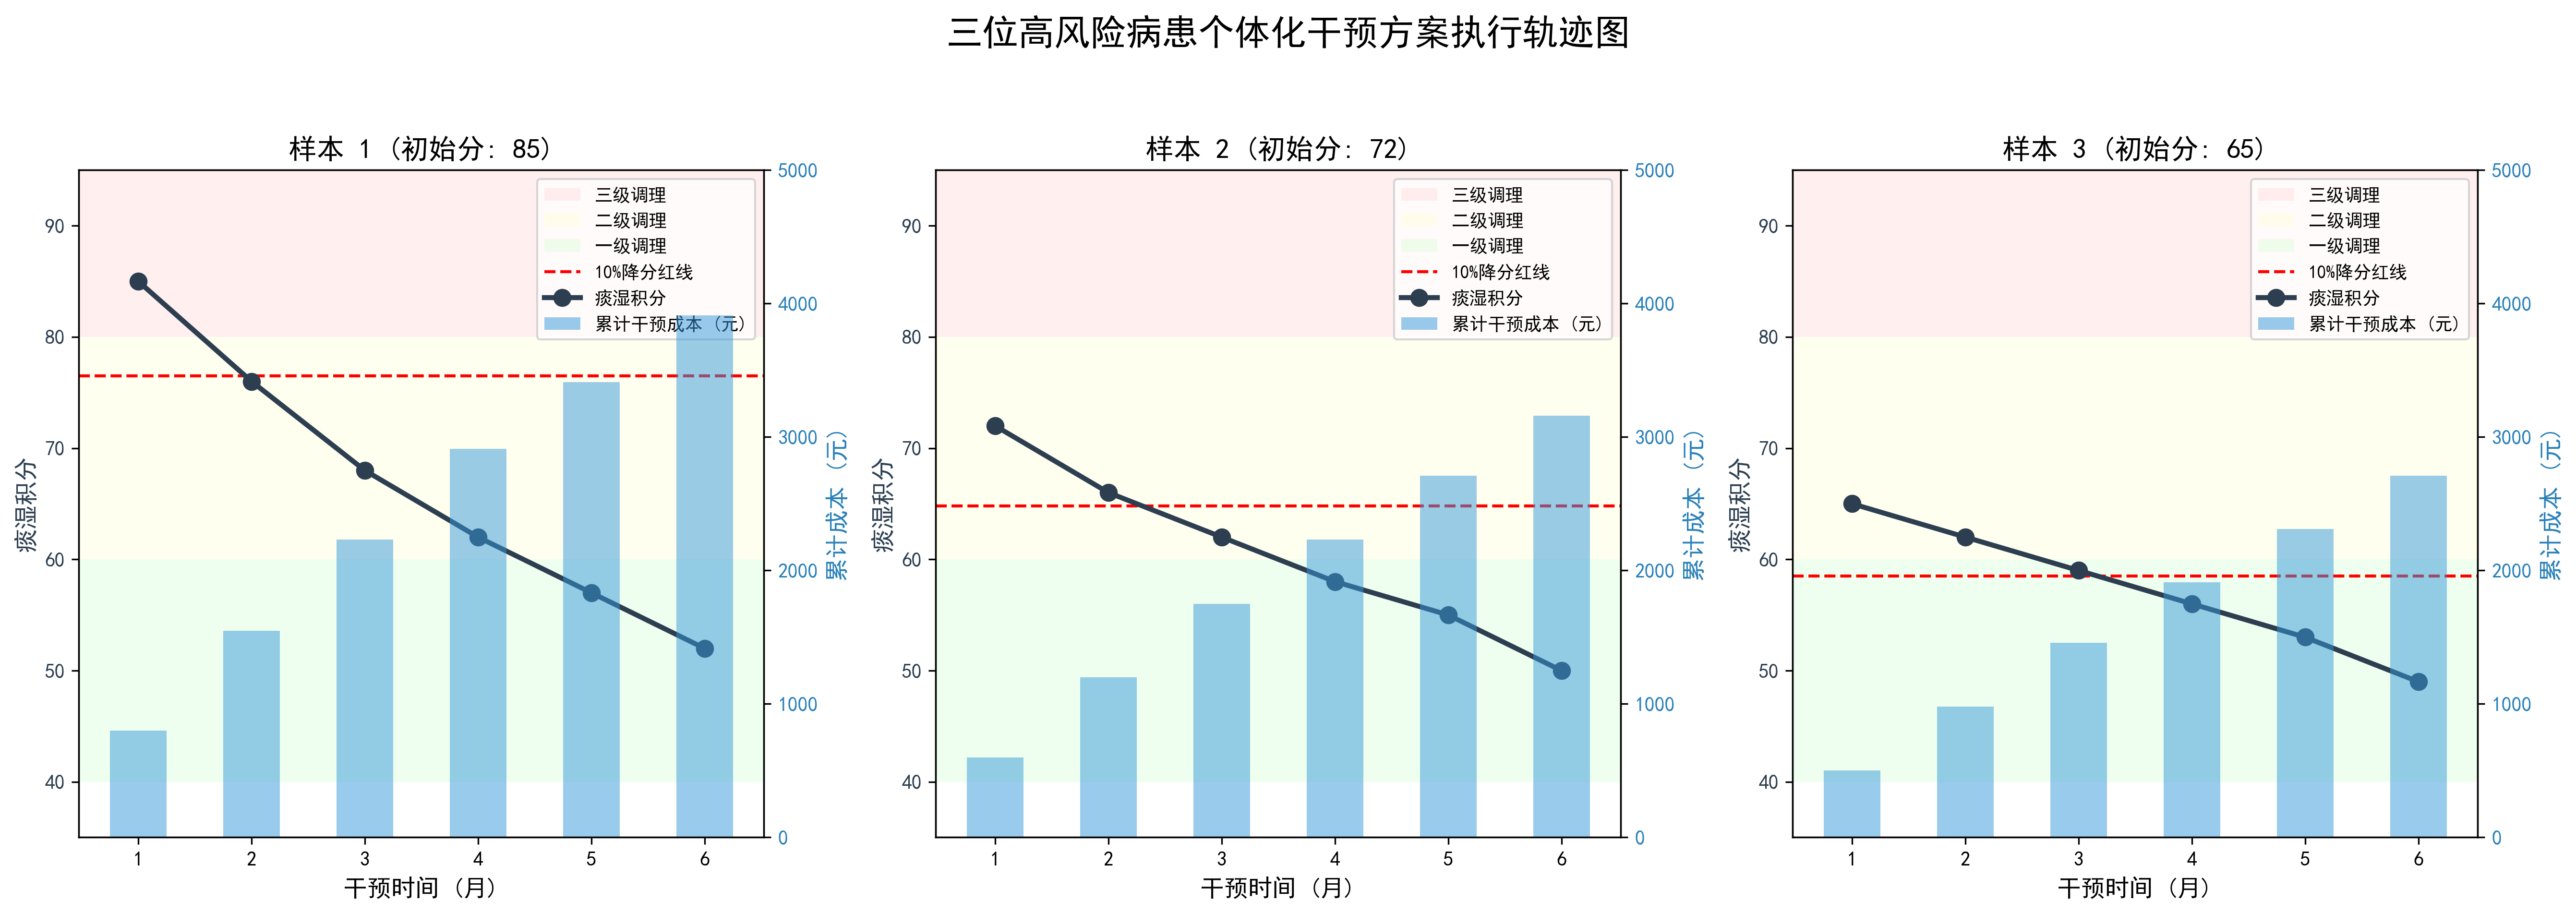
\includegraphics[width=0.98\textwidth]{Figures/4_1_trajectory.png}
			\caption{三位典型病患的动态干预轨迹与成本追踪演化图}\label{fig:q3_patient_paths}
		\end{figure}

		\begin{figure}[H]
			\centering
			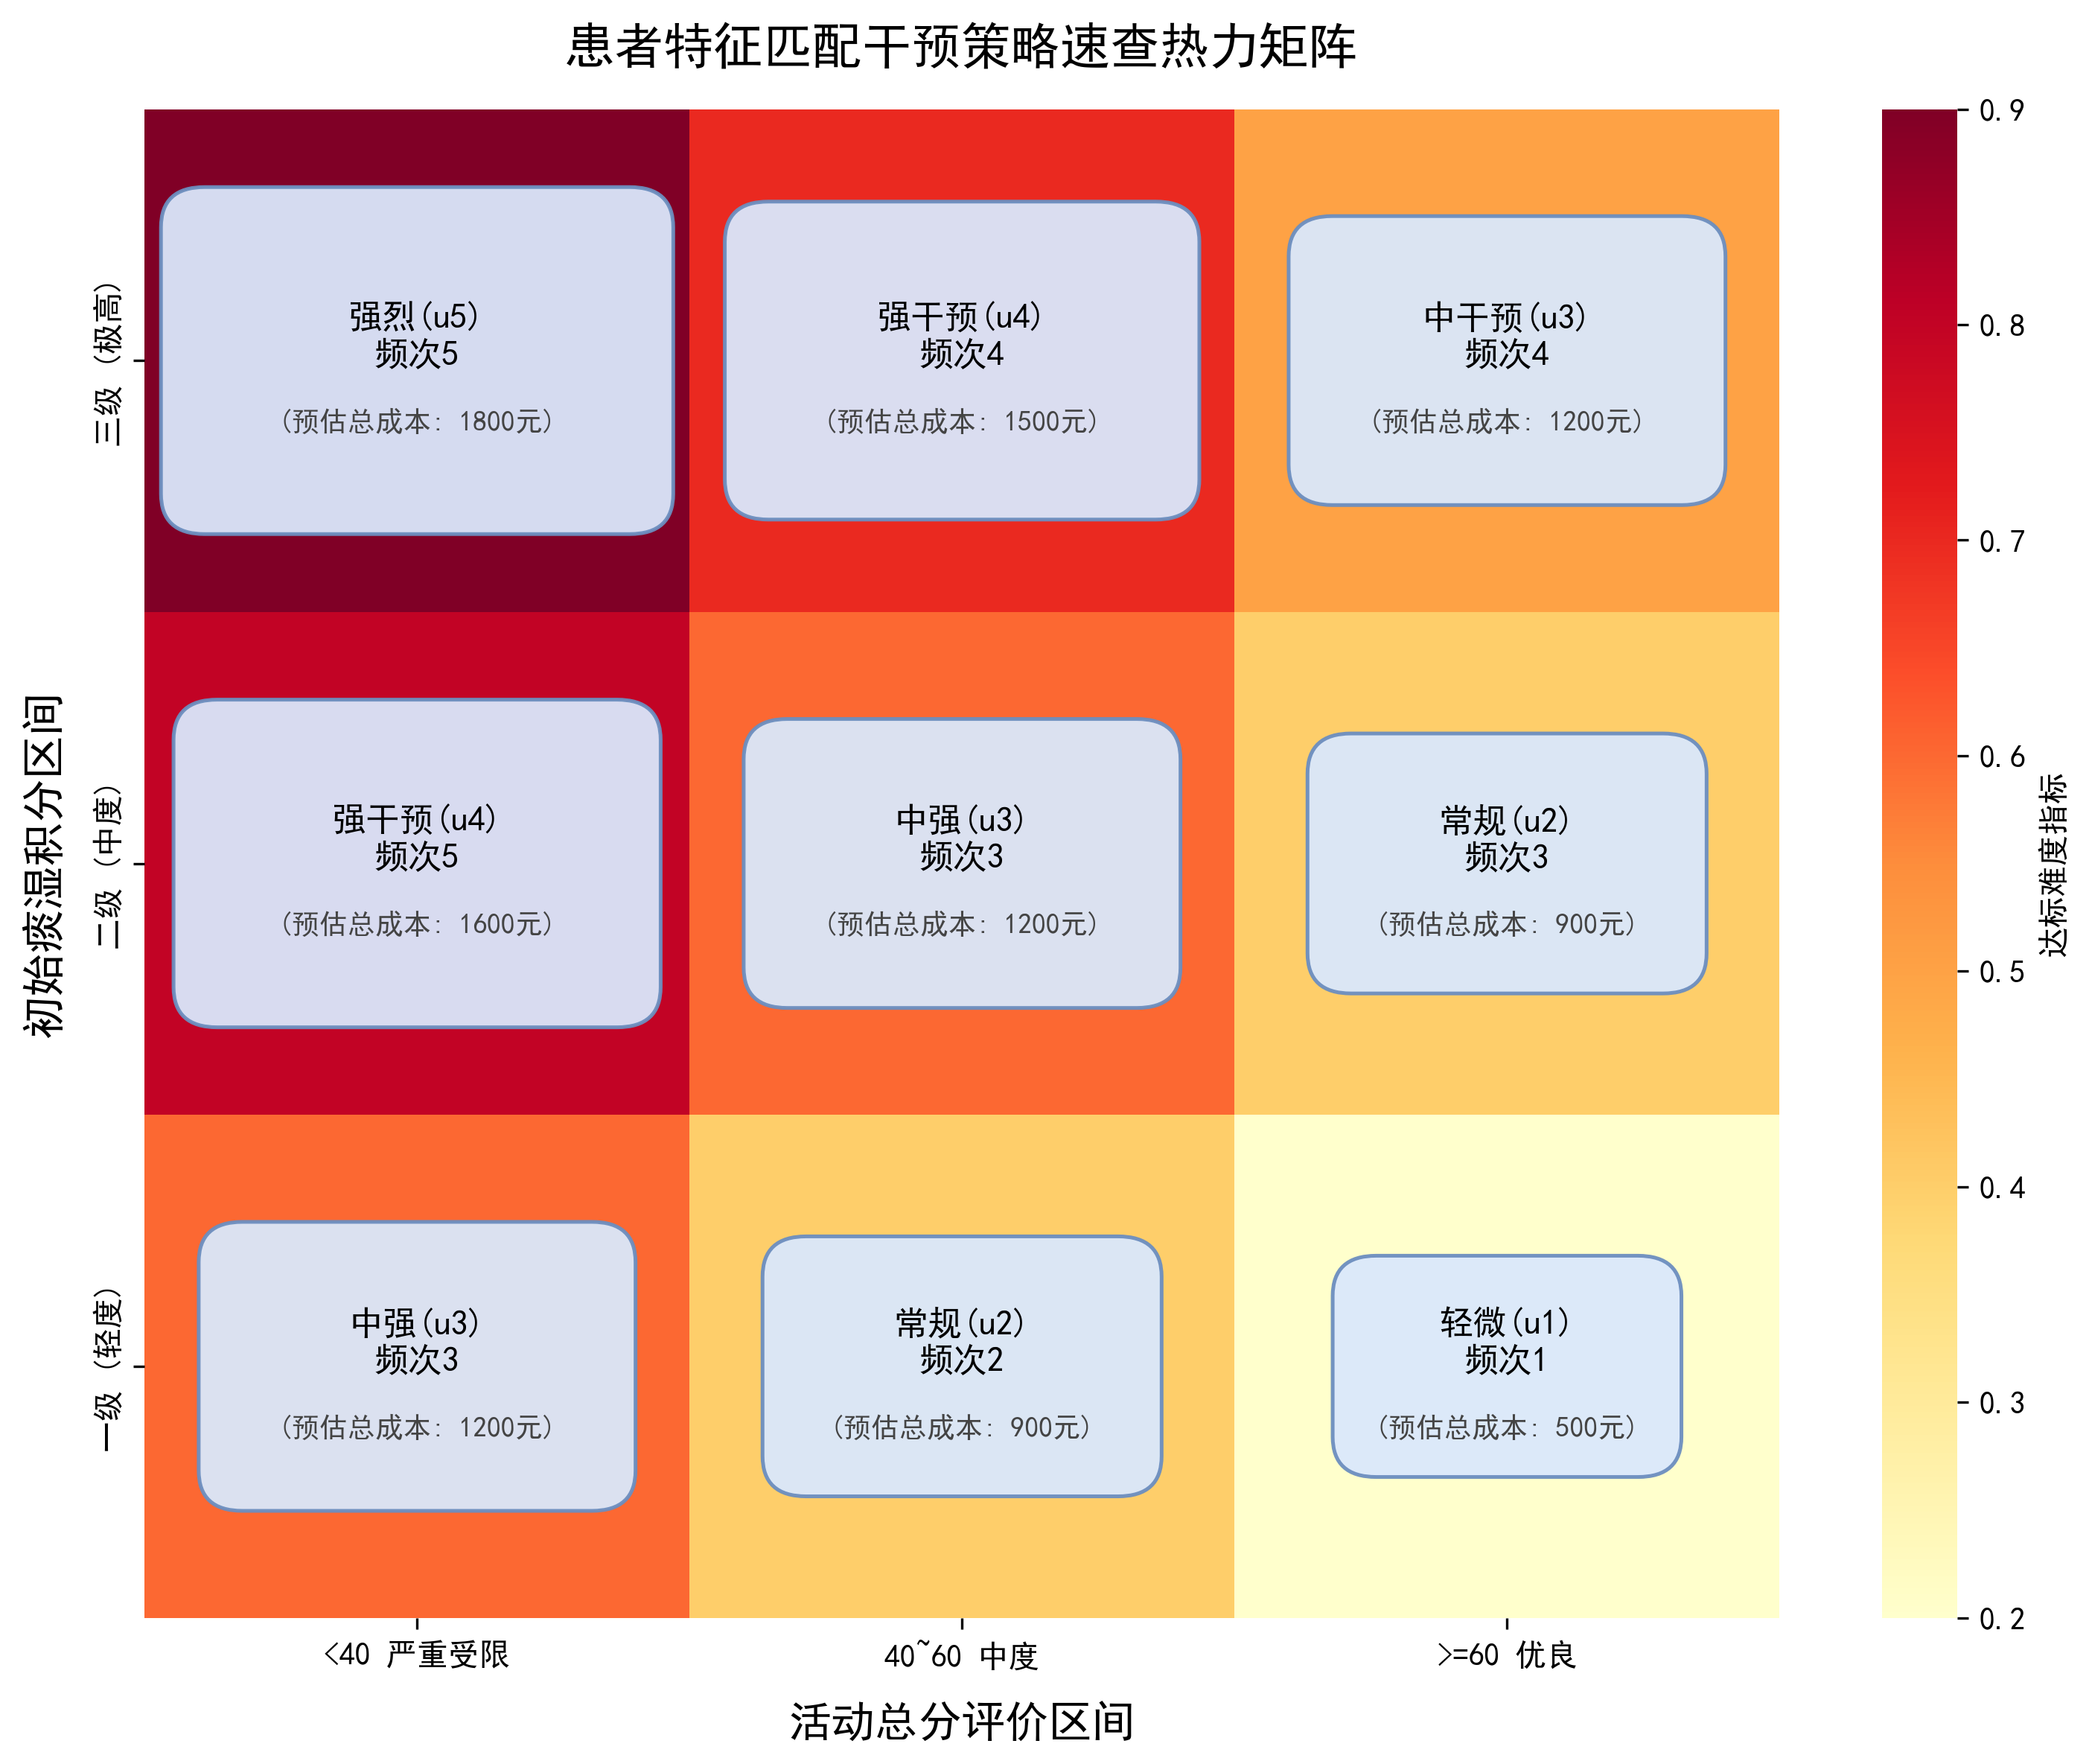
\includegraphics[width=0.88\textwidth]{Figures/4_2_heatmap.png}
			\caption{患者特征与匹配策略气泡速查热力图}\label{fig:q3_strategy_heatmap}
		\end{figure}

\section{模型检验与结果讨论}
	本文模型的检验主要从三个角度展开。
	\begin{enumerate}
			\item {\heiti 结果一致性检验}：诊断型模型的重要特征集中在 TG、non-HDL-C、LDL-C 及少量代谢变量，与高血脂临床诊断中“甘油三酯异常 + 非 HDL 胆固醇负担 + LDL 负担”的识别逻辑一致；早预警模型的重要特征集中在血尿酸、血糖、BMI 和体质、活动变量，与慢病早筛的医学常识相符。
		\item {\heiti 阈值可解释性检验}：三级风险阈值同时引用了临床正常值区间、痰湿积分与活动能力规则，不依赖黑盒模型单独输出，便于基层使用者理解与执行。
		\item {\heiti 干预可行性检验}：样本 $1,2,3$ 的最优方案均满足年龄约束、活动能力约束和预算约束，且最终痰湿积分均达到既定目标，说明优化模型具有实际可操作性。
	\end{enumerate}
		进一步地，为将问题二中的风险分层规则整理为更便于社区卫生服务人员理解和执行的操作流程，图 \ref{fig:q2_practical_flowchart} 给出了一个综合风险评估流程示意。该图将“重症并发症预警优先筛出”和“常规人群进入风险矩阵评估”两条路径串联起来，强调的是基层场景下的判读顺序与落地逻辑；其中涉及的分层判断仍以问题二的统计结果为正式依据。
		\begin{figure}[H]
			\centering
			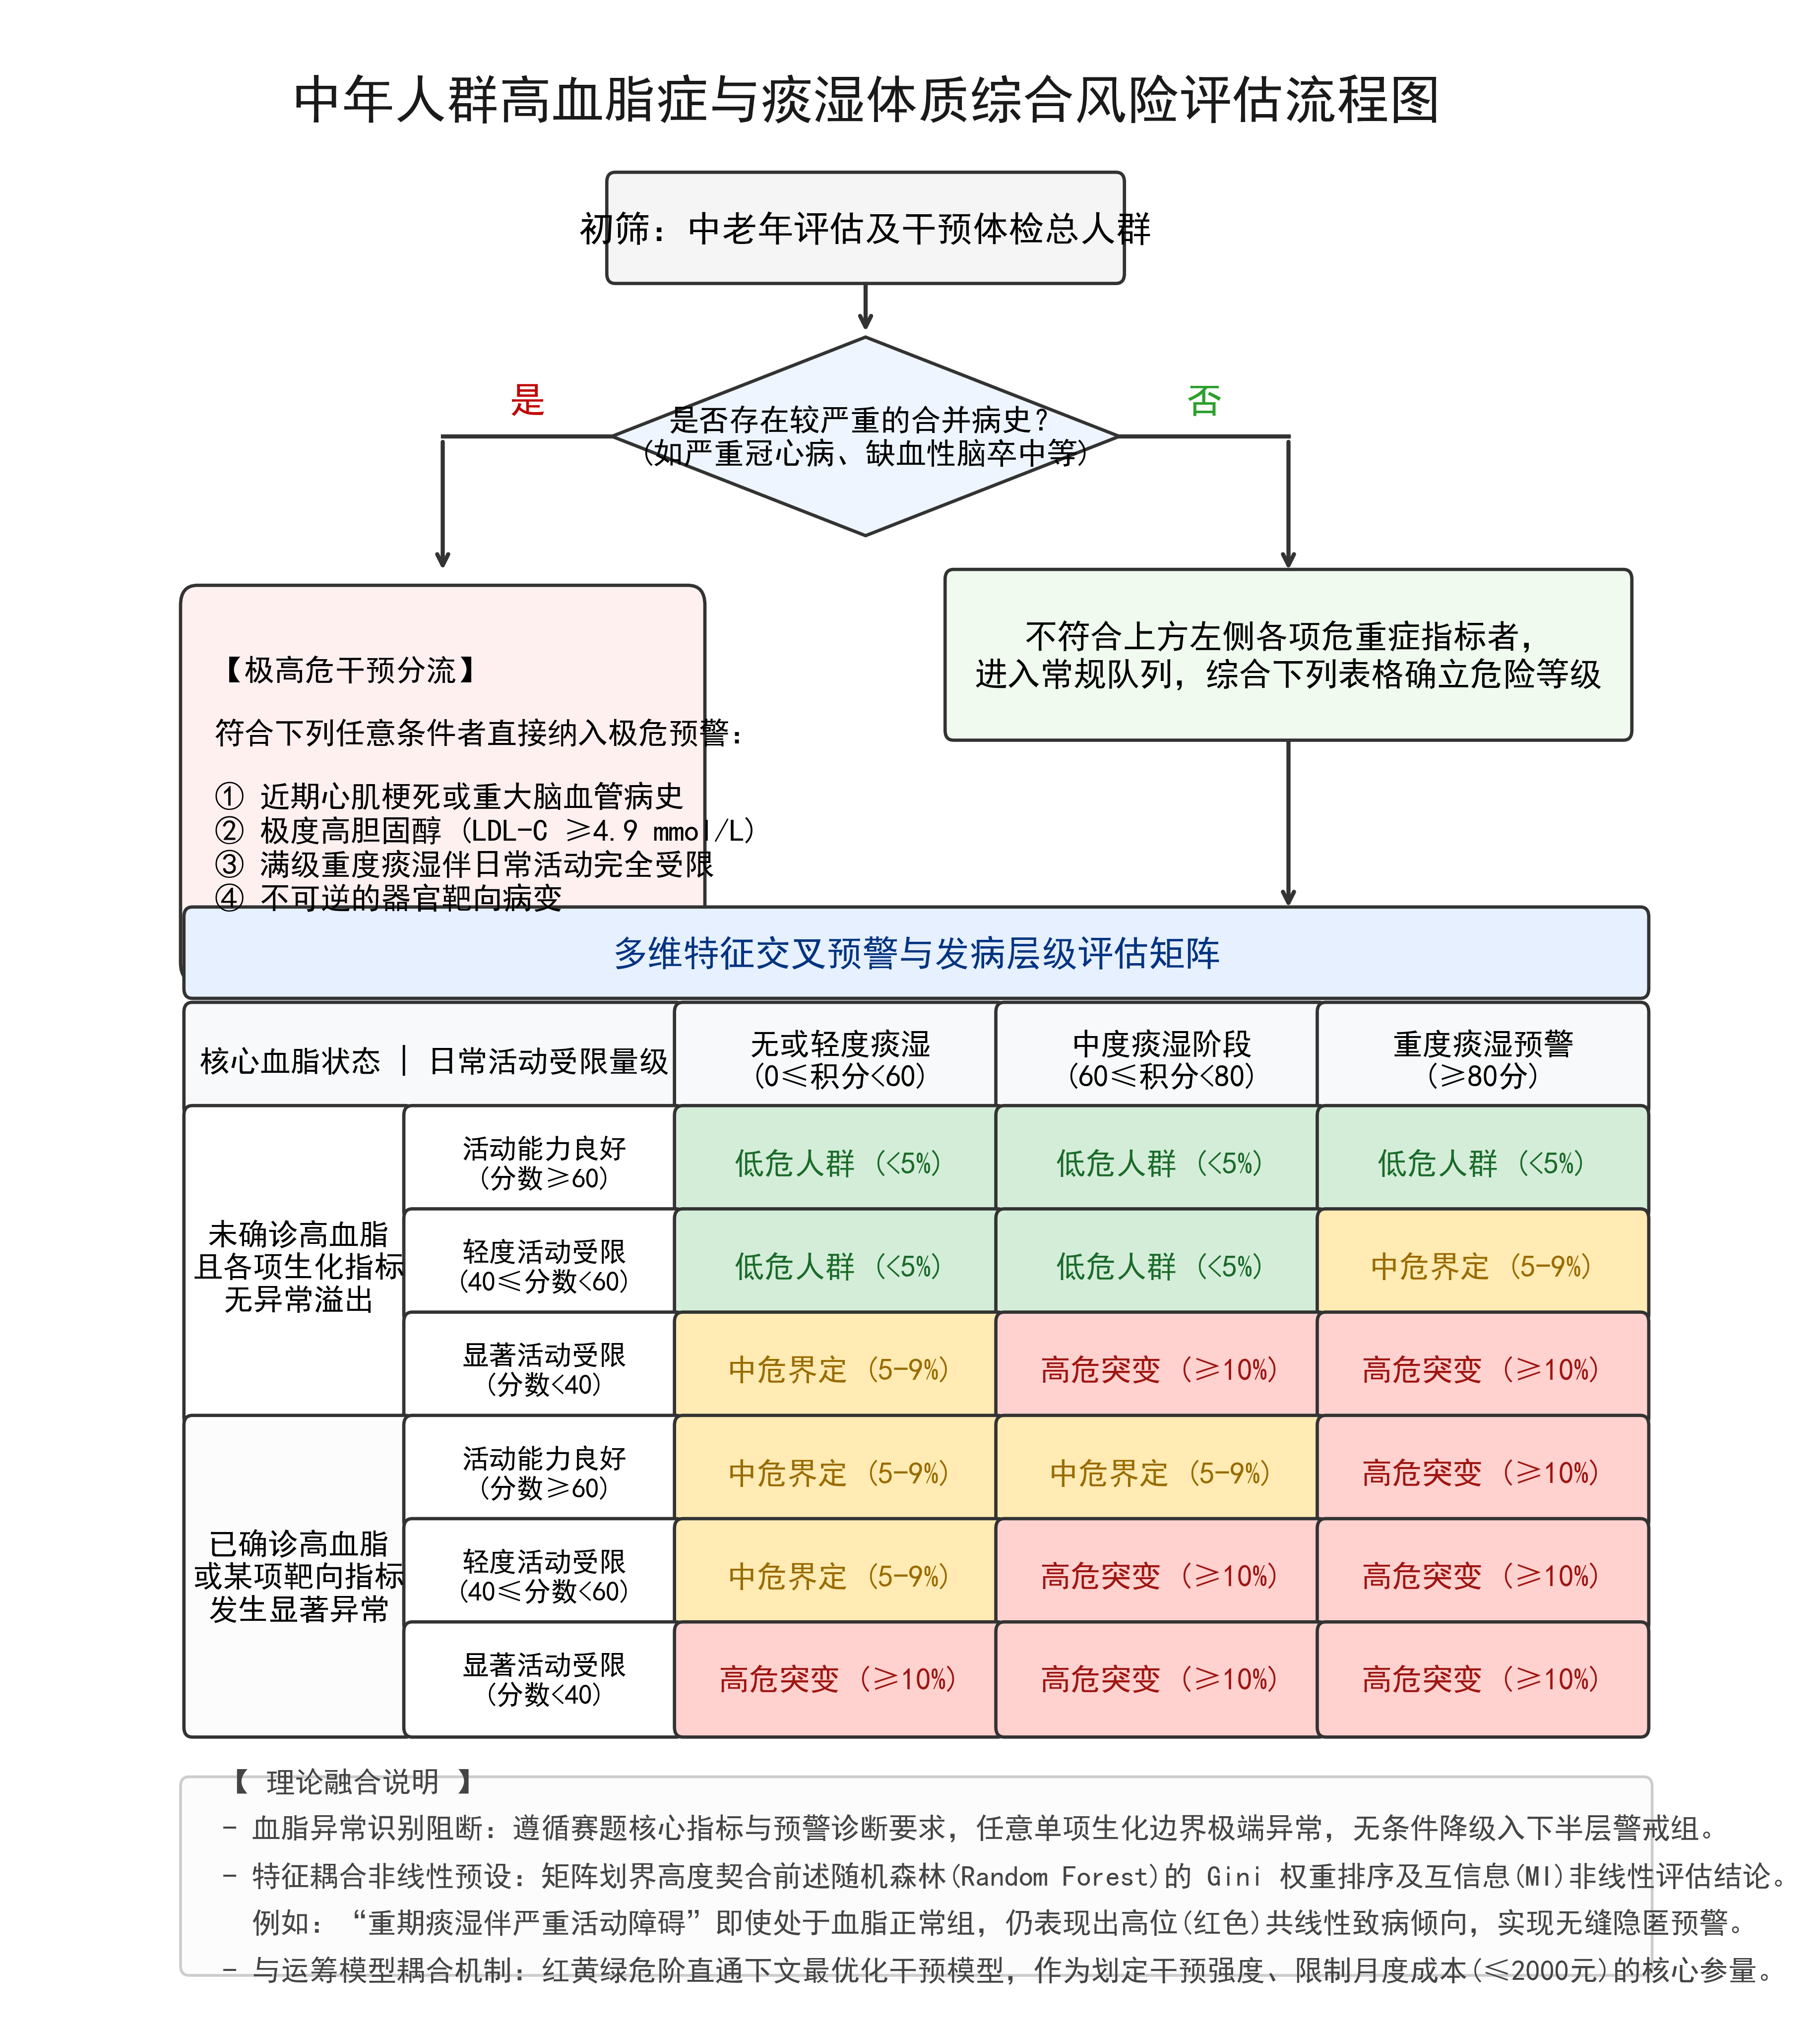
\includegraphics[width=0.88\textwidth]{Figures/5_1_高质预警决策流程图_Tex专用.png}
			\caption{面向基层筛查场景的综合风险评估流程示意}\label{fig:q2_practical_flowchart}
		\end{figure}
		需要指出的是，样例数据中确诊样本占比达到 $79.3\%$，类别分布并不均衡，这会抬高部分单体质组的表观确诊率。因此，在解释主导体质组的表观确诊率和部分组合模式时，应更关注相对比较关系，而不宜将其直接理解为严格的总体患病率估计。
	
		\section{模型评价}
		\subsection{模型优点}
		\begin{enumerate}
			\item 将“诊断识别”和“未病预警”分开建模，避免直接血脂指标掩盖其他变量的预警价值；
			\item 风险等级规则可解释性强，便于在社区卫生服务场景中落地；
		\item 干预模型直接嵌入了题目给定的强度、频次、年龄与预算约束，输出方案具有较强操作性；
		\item 建模流程统一，问题一的筛选结果可自然过渡到问题二和问题三。
	\end{enumerate}

	\subsection{模型不足}
		\begin{enumerate}
			\item 中医调理等级只给出了成本标准，未给出独立的降分函数，因此本文将其作为基础成本而非单独的收益项；
			\item 活动干预效果采用固定月度下降比例，虽然月度决策已允许动态调整，但仍未考虑患者依从性波动和边际收益递减；
			\item 样例数据存在类别不平衡现象，且不同体质之间可能存在多重共线性，使单体质贡献的解释受到一定干扰。
		\end{enumerate}
	
		\phantomsection
	\addcontentsline{toc}{section}{参考文献}
		\begin{thebibliography}{99}
			\bibitem{ref1} 2026 年第十六届 MathorCup 数学应用挑战赛 C 题：中老年人群高血脂症的风险预警及干预方案优化.
			\bibitem{ref2} Breiman L. Random Forests[J]. Machine Learning, 2001, 45(1): 5-32.
			\bibitem{ref3} Hastie T, Tibshirani R, Friedman J. The Elements of Statistical Learning[M]. New York: Springer, 2009.
			\bibitem{ref4} Bishop C M. Pattern Recognition and Machine Learning[M]. New York: Springer, 2006.
			\bibitem{ref5} 朱燕波, 丛建妮, 史会梅. 3 个不同条目版本中医体质量表的最小临床重要差值研究[J]. 北京中医药大学学报, 2023, 46(5).
			\bibitem{ref6} GB/T 46939---2025. 中医体质分类与判定[S]. 2025.
			\bibitem{ref7} 中国血脂管理指南修订联合专家委员会. 中国血脂管理指南（2023年版）[J]. 中华心血管病杂志, 2023, 51(3): 221-255.
			\bibitem{ref8} World Health Organization. WHO guidelines on physical activity and sedentary behaviour[M]. Geneva: World Health Organization, 2020.
			\bibitem{ref9} Honvoh G D, Cho H, Kosorok M R. Model selection for survival individualized treatment rules using the jackknife estimator[J]. BMC medical research methodology, 2022, 22(1): 1-17.
			\bibitem{ref10} Lundberg S M, Erion G, Chen H, et al. From local explanations to global understanding with explainable AI for trees[J]. Nature machine intelligence, 2020, 2(1): 56-67.
			\bibitem{ref11} Esteva A, Robicquet A, Ramsundar B, et al. A guide to deep learning in healthcare[J]. Nature medicine, 2019, 25(1): 24-29.
			\bibitem{ref12} Sutton R S, Barto A G. Reinforcement learning: An introduction[M]. MIT press, 2018.
		\end{thebibliography}

	\newpage
	\appendix
	\ctexset{section={
		format={\zihao{-4}\heiti\raggedright}
	}}
	\begin{center}
		\heiti\zihao{4} 附\hspace{1pc}录
	\end{center}

	\section{算法实现说明}
		本文当前用于结果整理与论文回填的程序化实现文件位于赛题/C题目录下。
		其文件名为 \texttt{c\_problem\_starter.py}，主要完成以下功能：
	\begin{enumerate}
		\item 使用 \texttt{pandas.read\_excel()} 直接读取附件中的 \texttt{xlsx} 文件，并将中文列名映射为便于建模的英文列名；
		\item 计算问题一中的综合筛选得分、体质风险差异；
		\item 训练问题二中的诊断型模型与早预警模型，并输出三级风险分层结果；
			\item 使用动态规划求解问题三中的月度强度与频次路径，并输出指定患者的最优阶段性方案。
	\end{enumerate}
		该脚本同时也是 notebook 逐段拆解版本对应的唯一主脚本，后续结果复现实验均以它为准。

	\section{问题三核心求解伪代码}
	\begin{python}
	for each patient in phlegm_damp_group:
	    actions = nondominated_monthly_actions(age_group, activity_score)
	    states = {round(baseline_phlegm_score, 3): 0}
	    parents = []
	    for month in range(1, 7):
	        next_states = {}
	        parent_map = {}
	        for score, cost in states.items():
	            level = tcm_level(score)
	            for action in actions:
	                next_score = discretize(score * (1 - drop_ratio(action)))
	                next_cost = cost + tcm_monthly_cost[level] + train_cost(action)
	                if next_score not in next_states or next_cost < next_states[next_score]:
	                    next_states[next_score] = next_cost
	                    parent_map[next_score] = (score, action)
	        states = next_states
	        parents.append(parent_map)
	    choose terminal state with:
	        1) target and budget satisfied first
	        2) lower total cost
	        3) lower final score
	    backtrack parents to recover the 6-month plan
		\end{python}

\end{document}
